\apendice{Documentación técnica de programación}
\section{Introducción}
El manual de programador es una herramienta esencial para cualquier profesional que se dedique al desarrollo de software. Su objetivo principal es proporcionar información detallada y clara sobre el uso de un programa o aplicación, así como guías y recomendaciones para la resolución de problemas y situaciones que puedan surgir durante el proceso de programación.

Así, este manual le permitirá al programador ahorrar tiempo al consultar rápidamente la información necesaria en lugar de tener que buscarla en diferentes fuentes, así como también reducir los errores y los problemas de compatibilidad, ya que proporciona una guía clara sobre el uso adecuado de las herramientas y los recursos disponibles. De igual forma, permite optimizar la calidad del software desarrollado, ilustrando sobre las mejores prácticas y los estándares de calidad que deben seguirse durante el proceso de programación. 

Tal es el caso del presente Manual de Programador en el que se indican los pasos a seguir para el despliegue del backend desarrollado en este TFG que dará lugar a la futura aplicación móvil, dirigida a personas afectadas por la EM, en su intención de ayudarles a navegar por el sistema de salud y autogestionar su enfermedad desde el momento en que son diagnosticadas.

En este sentido, a continuación, se explican las diferentes etapas para el despliegue del backend en un servidor, así como también las herramientas con las que se deberá trabajar para realizar cualquier tipo de mantenimiento o desarrollar nuevas funcionalidades.

\subsection{Infraestructura}\label{infraestructura}
El backend debe estar alojado en un servidor web. En este caso se seleccionó Digital Ocean.

Digital Ocean es una plataforma de alojamiento en la nube que ofrece la posibilidad de crear y administrar maquinas virtuales, en adelante Droplets, así como otros servicios relacionados con la infraestructura en la nube; proporciona un entorno seguro y escalable para la implementación de aplicaciones web y móviles \cite{web:docker}.

\subsubsection{Creación de cuenta}
 El primer paso a seguir para utilizar la plataforma es el registro y creación de usuario. Para ello debemos dirigirnos al sitio web de la plataforma ingresando al siguiente enlace: \href{https://www.digitalocean.com/}{Digital Ocean}.

Una vez dentro del sitio, y encontrándose en la página de inicio, se debe hacer clic en la opción de Sign Up (Registrarse, en español), ubicada en la parte derecha de la misma. Está opción nos llevará a la sección donde nos registramos utilizando nuestro correo electrónico (ver figura~\ref{Img:Web+Digital+Ocean}).

\begin{figure}[h]
    \centering
    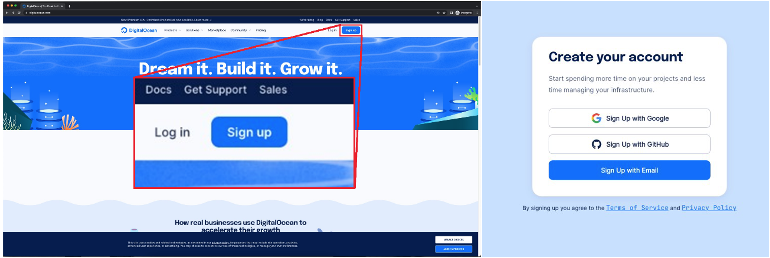
\includegraphics[width=0.9\textwidth]{img/infraestructura/pagina_digital_ocean.png}
    \caption{Creación de usuario en DigitalOcean.} \label{Img:Web+Digital+Ocean}
\end{figure}

Se debe hacer clic en la tercera opción marcada en azul, Sing Up with email, la que nos permitirá ingresar con un usuario y correo sin necesidad de usar sistemas de Single Sign On, como lo son Google o Github (ver figura~\ref{Img:Web+Registro+en+Digital+Ocean}).

\begin{figure}[h]
    \centering
    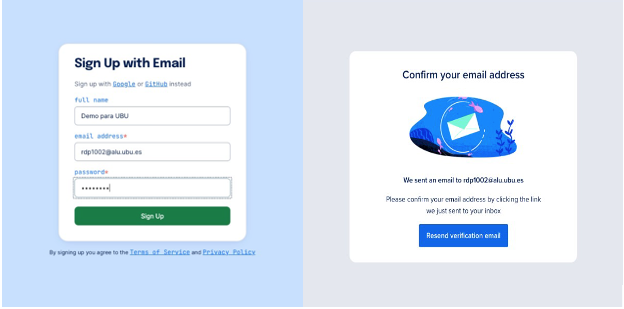
\includegraphics[width=0.9\textwidth]{img/infraestructura/pagina_de_registro.png}
    \caption{Registro y confirmación de email.} \label{Img:Web+Registro+en+Digital+Ocean}
\end{figure} 

\newpage

Una vez que rellenamos los datos que nos solicita la plataforma, ésta nos enviará un código de confirmación por email para comprobar que hemos sido nosotros quienes creamos la cuenta (ver figura~\ref{Img:Web+Registro+en+Digital+Ocean}). En este punto tendremos que abrir nuestro correo electrónico en la plataforma que corresponda, acceder al mail que hayamos recibido de Digital Ocean para verificar nuestra identidad, y luego hacer clic en el enlance que se nos suministra para confirmar la cuenta.\\
Habiendo completado el paso anterior, la plataforma nos solicitará dar de alta una tarjeta de crédito, o asociar una cuenta de Paypal, para poder realizar los pagos mensuales correspondientes al uso del servicio. Además, es importante destacar que Digital Ocean solicita realizar una recarga inicial de 5, 10 o 20 dólares americanos para poder comenzar a utilizar los servicios; una vez realizado este pago la plataforma cobrará a mes vencido.

\subsubsection{Creación de Droplet}

Luego de completar el registro e iniciar sesión en la plataforma, pasamos a la creación del Droplet. Un Droplet es un servidor virtual independiente que se puede configurar para realizar una variedad de tareas; es una combinación de recursos informáticos, como RAM, CPU y almacenamiento, que se pueden escalar vertical u horizontalmente según las necesidades del usuario \cite{web:digitalocean}. Por otra parte, un servidor virtual es un software que simula el hardware de una computadora y permite que múltiples sistemas operativos compartan los recursos de una sola máquina física \cite{web:vps}.

Así, en Digital Ocean las instancias de máquinas virtuales son llamadas Droplet, y cada una tiene ciertas características de acuerdo con el propósito con el que se utilizará el mismo. En nuestro caso, usaremos un Droplet de propósito general, con un costo de 7 dólares por mes, para comenzar a trabajar dado que permite escalar el sistema en un futuro, si lo necesitamos. Asimismo, el Droplet de propósito general ofrece una amplia gama de opciones de configuración. Para crear el Droplet, seguiremos los pasos descriptos a continuación. 

Estando dentro de nuestro perfil en Digital Ocean, hacemos clic en la opción Create, en la parte superior derecha, y luego seleccionamos la opción Droplets que nos llevará a la siguiente sección en donde debemos elegir la zona geográfica, sistema operativo y el tipo de Droplet a crear (ver figura~\ref{Img:Web+Creación+de+droplet+en+Digital+Ocean}). 

\begin{figure}[h]
    \centering
    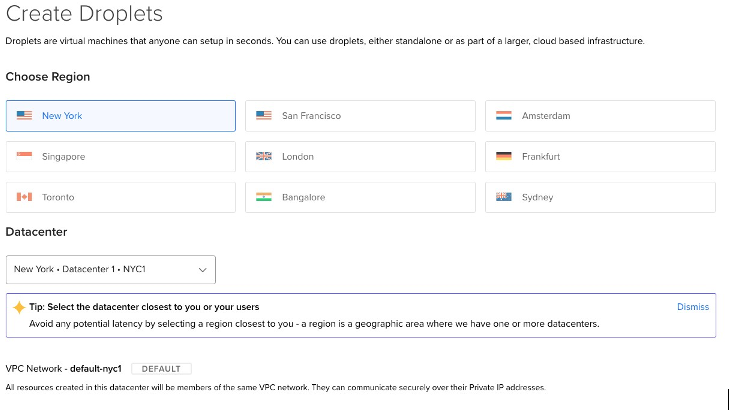
\includegraphics[width=0.9\textwidth]{img/infraestructura/crear-droplet.png}
    \caption{Crear droplet} \label{Img:Web+Creación+de+droplet+en+Digital+Ocean}
\end{figure} 

En nuestro caso, hemos seleccionado Nueva York (por tratarse del área más cercana a Latinoamérica) y, en lugar de trabajar con una máquina con el sistema operativo, hemos seleccionado desde el Marketplace una imagen precreada de Docker, que integra también Docker Compose.

Lo anterior responde a un uso inteligente de los recursos existentes para evitar instalar Docker manualmente y evitar posibles fallos durante dicho proceso.

Amerita explicitar que Docker es una plataforma de software que permite la creación, el despliegue y la ejecución de aplicaciones en contenedores, mientras que un contenedor es un ambiente de software que ofrece todo lo necesario para ejecutar una aplicación, incluyendo el código, las bibliotecas y las herramientas del sistema \cite{web:docker}. Por otro lado, Docker Compose es una herramienta que permite definir y ejecutar aplicaciones Docker compuestas por múltiples contenedores \cite{web:docker-compose}. 

\subsubsection{Creación de SSH KEY}

En lo referente a la seguridad, se puede establecer que, para acceder al Droplet, se deba utilizar bien sea una contraseña o una llave SSH KEY, siendo esta última opción la utilizada. Una SSH KEY es una clave criptográfica utilizada para autenticación y encriptación en la comunicación segura a través del protocolo SSH, referido al acceso a un servidor mediante el uso de un canal seguro que permite a un usuario autenticarse en un servidor remoto, sin tener que ingresar una contraseña cada vez que se inicia sesión \cite{web:ssh-key}.

Para agregar una SSH KEY a Digital Ocean seleccionamos esta opción cuando creamos el Droplet marcando New SSH KEY en la sección Choose authentication method. En este punto, se nos desplegará un modal que nos permitirá agregar nuestra SSH Key personal, la que debemos haber creado previamente (ver figura~\ref{Img:Web+Método+de+autenticación+SSH+KEY}).


\begin{figure}[h]
    \centering
    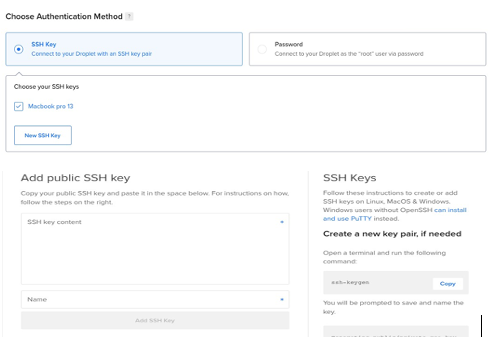
\includegraphics[width=0.8\textwidth]{img/infraestructura/ssh-key.png}
    \caption{Método de autenticación SSH KEY} \label{Img:Web+Método+de+autenticación+SSH+KEY}
\end{figure} 


Si en nuestra computadora no tenemos una clave generada previamente del tipo SSH KEY procederemos a generarla abriendo la terminal de comandos en el sistema operativo. En el caso de las computadoras MAC con sistema operativo OSX, para abrir la terminal se debe presionar el atajo de teclado cmd + barra espaciadora. Luego, debemos ingresar el siguiente comando: ssh-keygen, y enseguida la consola preguntará si le queremos dar un nombre y si se desea agregar una contraseña a la llave (ver figura~\ref{Img:Creación+de+SSH+KEY+en+MAC}).

\begin{figure}[h]
    \centering
    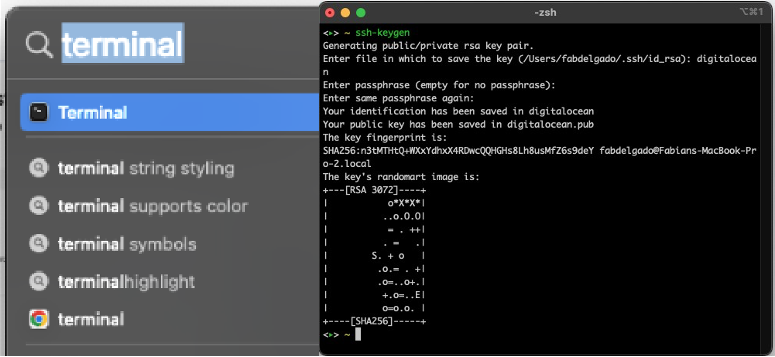
\includegraphics[width=0.8\textwidth]{img/infraestructura/crear-ssh-key-mac.png}
    \caption{Creación de SSH KEY en MAC} \label{Img:Creación+de+SSH+KEY+en+MAC}
\end{figure} 


Una vez finalizado este proceso, debemos copiar la llave generada en Digital Ocean, para lo cual nos dirigimos al directorio donde se guardan todas las llaves: cd/Users/fabdelgado/.ssh/. Una vez en el directorio, ejecutamos el comando “ls” para ver todas las llaves generadas y encontrar la que necesitamos. Luego, para copiar la clave generada ejecutamos el comando “cat digitalocean.pub” (ver figura~\ref{Img:Copiado+de+clave+generada}). Es de tener en cuenta que se debe realizar con la llave en la extension .pub por ser ésta la clave pública.

\begin{figure}[h]
    \centering
    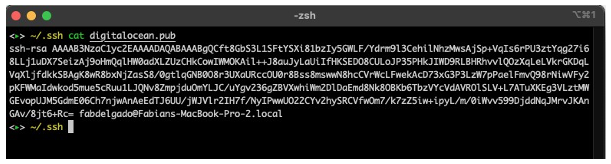
\includegraphics[width=0.7\textwidth]{img/infraestructura/copiado-ssh-key.png}
    \caption{Copiado de clave generada.} \label{Img:Copiado+de+clave+generada}
\end{figure} 

Una vez copiado el contenido de la clave pública procedemos a ingresarla en la cuenta de Digital Ocean y darle un nombre para guardarla en la plataforma. Finalmente, presionamos Add SSH Key y de esta forma ya nos queda disponible para futura creación de otros Droplets (ver figura~\ref{Img:Agregar+SSH+KEY+en+DigitalOcean}).

\newpage
\begin{figure}[h]
    \centering
    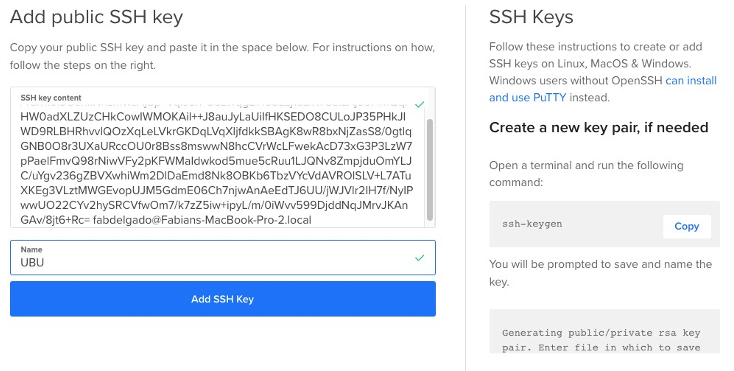
\includegraphics[width=0.7\textwidth]{img/infraestructura/agregar-ssh-key-digital-ocean.png}
    \caption{Agregar SSH KEY en DigitalOcean.} \label{Img:Agregar+SSH+KEY+en+DigitalOcean}
\end{figure} 


\subsubsection{Creación de base de datos}
Para la creación de la base de datos también se utiliza un servicio ofrecido por Digital Ocean a este respecto. Ello brinda alta disponibilidad y permite despreocuparnos del mantenimiento y los respaldos diarios a realizar.
Para crear una nueva instancia de base de datos se hace clic en el botón Create, y se selecciona la opción Databases, que redirige a una página para establecer la configuración de la instancia que deseamos crear. En nuestro caso seleccionamos la región por defecto de Nueva York para tener menos latencia con el Droplet previamente creado, y como motor de base de datos seleccionamos PosgretSQL en el plan starter (ver figura~\ref{Img:Creación+de+base+de+datos en+DigitalOcean}).
\begin{figure}[h]
    \centering
    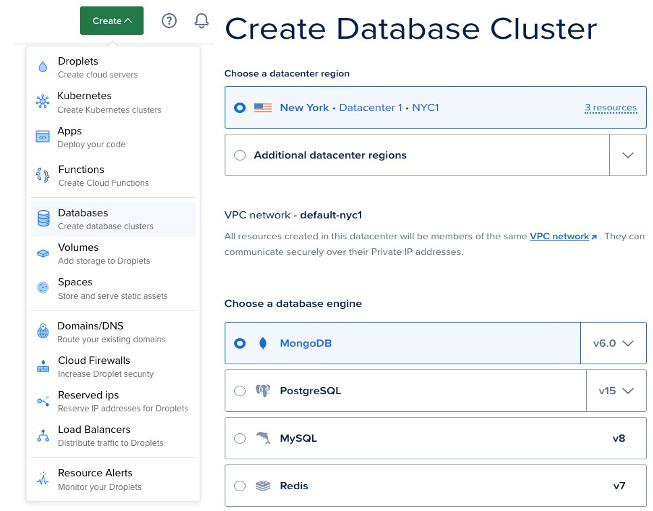
\includegraphics[width=0.6\textwidth]{img/infraestructura/crear-base-de-datos.png}
    \caption{Creación de base de datos en DigitalOcean.} \label{Img:Creación+de+base+de+datos en+DigitalOcean}
\end{figure} 


En relación con lo anterior, PostgreSQL es un sistema de gestión de bases de datos ORDBMS (Object-Relational Database Management System) de código abierto y de alta performance, que utiliza un modelo cliente-servidor, siendo, además, altamente escalable. PostgreSQL posee una arquitectura modular, lo que significa que los módulos pueden ser añadidos o eliminados a medida que las necesidades van mutando \cite{web:postgresql}.
Para finalizar, debemos indicar el nombre que deseamos colocar para la instancia, y seleccionar el proyecto al que queremos que esté relacionado, que en este caso es el llamado EMUR. Así, luego de confirmar la creación, ya nos aparece en nuestro panel de proyecto, siendo el siguiente paso la creación del usuario con el que nos conectaremos a la base de datos donde se guarda la información. 
En este sentido, para configurar el usuario y la base de datos debemos dirigirnos al apartado Users and Databases, en el que crearemos un usuario llamado EMUR, una base de datos para desarrollo y una para producción llamada Backend (ver figura~\ref{Img:Configuración+de+usuario+en PostgreSQL}).

\begin{figure}[h]
    \centering
    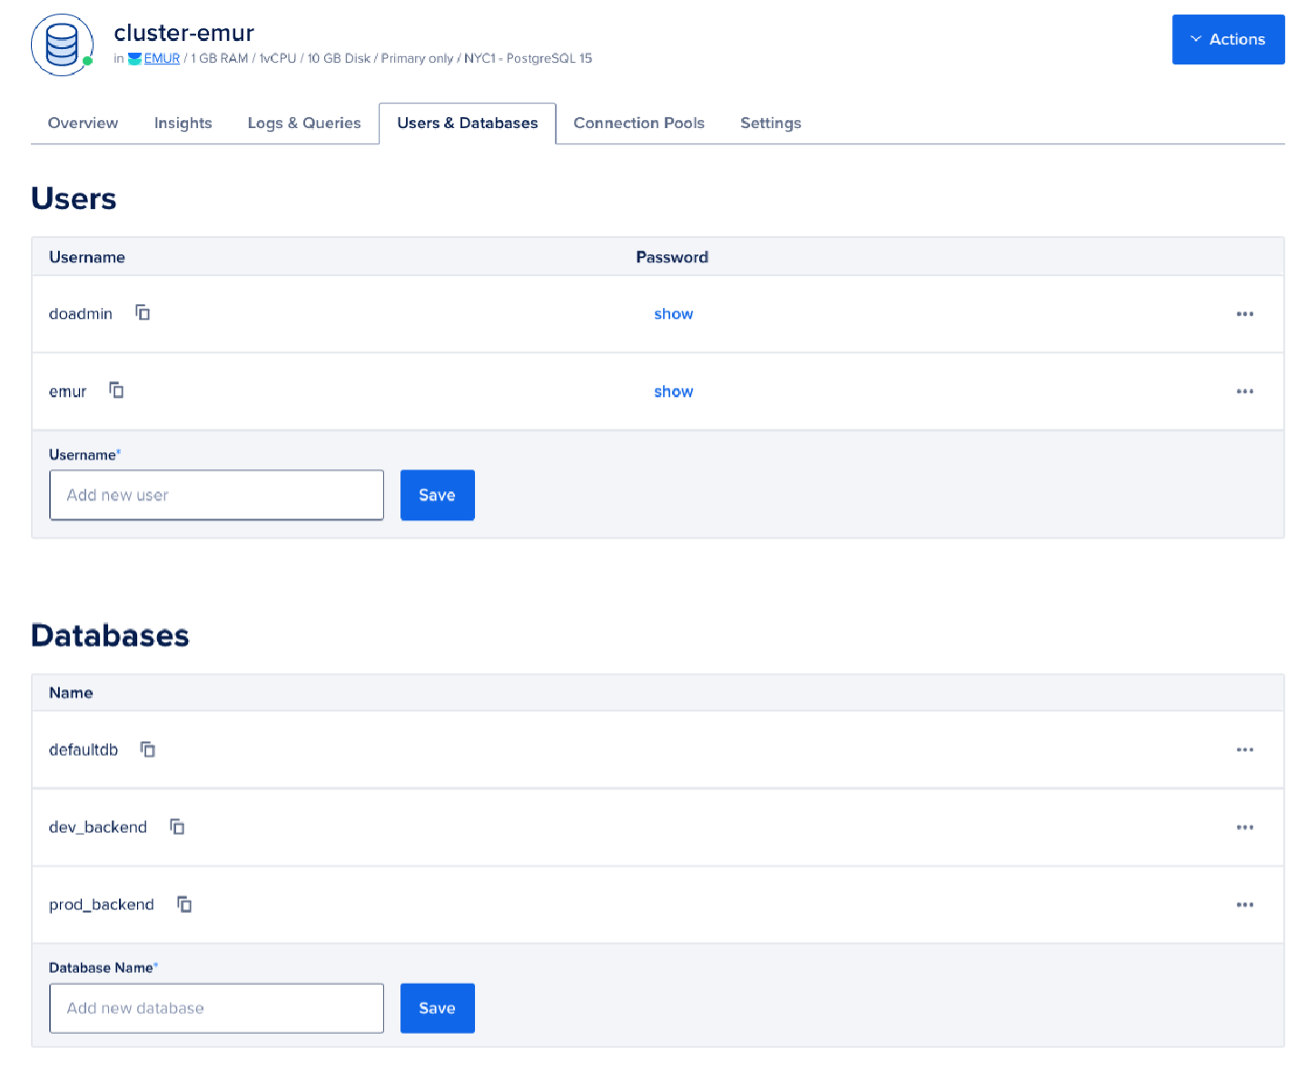
\includegraphics[width=0.9\textwidth]{img/infraestructura/cluster-db-digital-ocean.png}
    \caption{Configuración de usuario en PostgreSQL.} \label{Img:Configuración+de+usuario+en PostgreSQL}
\end{figure} 


\subsection{}{SonarQube}

SonarQube es una herramienta de análisis estático de código que permite detectar problemas y vulnerabilidades en el código fuente; es una herramienta efectiva para medir la calidad del código que proporciona una gran cantidad de métricas que permiten evaluar la complejidad, legibilidad y mantenibilidad del código \cite{web:sonarqube}. En este sentido, luego de realizar una análisis comparativo de costos, contrastando el costo de tener un servidor dedicado para utilizar SonarQube contra la opción de usar la versión hosteada por SonarQube, se decide optar por la versión en la nube de SonarCloud de más bajo coste (ver tabla~\ref{tab:requisitos-sonar}).

\begin{table}[H]
\centering
\begin{tabular}{ll}
\toprule
Plataforma                     & Precio                           \\
\midrule
\texttt{Digital Ocean SonarQube}       & 12 USD              \\
\texttt{SonarQube Cloud}      & 10 USD             \\
\bottomrule
\end{tabular}
\caption{Comparativa de precios SonarQube}
\label{tab:requisitos-sonar}
\end{table}

Para crear el usuario en SonarCloud se utiliza el Single Sign On de Github que condice con el hecho de que nuestro proyecto se encuentra en esta plataforma y nos resultará más fácil su integración.\\

Para crear un proyecto en SonarCloud debemos de usar la opción Import an organization from GitHub (ver figura~\ref{Img:Registro+en+SonarCloud}).
\begin{figure}[h]
    \centering
    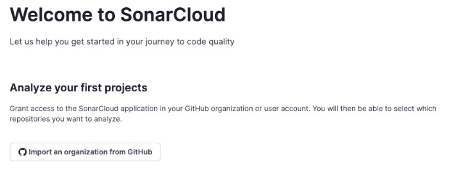
\includegraphics[width=0.9\textwidth]{img/infraestructura/registro-sonarcloud.png}
    \caption{Registro en SonarCloud.} \label{Img:Registro+en+SonarCloud}
\end{figure} 

Luego de esto, el siguiente paso será seleccionar la organización a sincronizar, en este caso EMUR-UY, para después indicar si vamos a otorgar permisos sobre todos los repositorios o sólo algunos. Para el caso que nos convoca, seleccionaremos Only select repositories, lo cual nos permite tener un control más detallado sobre los proyectos que queremos importar para analizar, y por último pulsamos Install (ver figura~\ref{Img:Configuracion+de+SonarCloud}).

\begin{figure}[h]
    \centering
    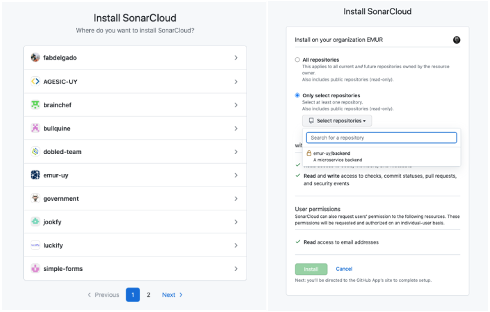
\includegraphics[width=0.9\textwidth]{img/infraestructura/configurar-sonar-cloud.png}
    \caption{Configuracion de SonarCloud.} \label{Img:Configuracion+de+SonarCloud}
\end{figure} 
\newpage

Seguidamente, SonarCloud, nos solicita crear una organización (ver figura~\ref{Img:Crear+organización}), donde nos pide ingresar email, identificador de proyecto y tipo de plan, para después solicitar la información de pago y el tipo de uso, y así proceder con la creación del proyecto. 

\begin{figure}[h]
    \centering
    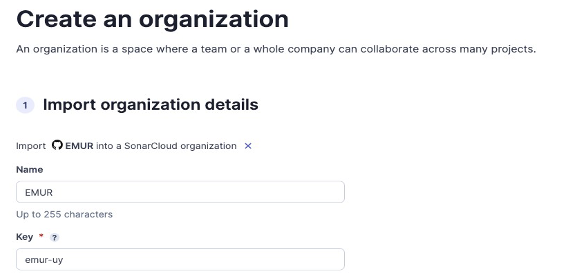
\includegraphics[width=0.7\textwidth]{img/infraestructura/crear-organizacion.png}
    \caption{Crear organización.} \label{Img:Crear+organización}
\end{figure} 

Tras realizar todas estas precisiones procedemos a configurar el proyecto que necesitamos escanear haciendo clic en Set Up, con lo que SonarCloud comenzará a analizar todo el repositorio (ver figura~\ref{Img:Configuración+de+análisis+de+proyectos}).

\newpage
\begin{figure}[h]
    \centering
    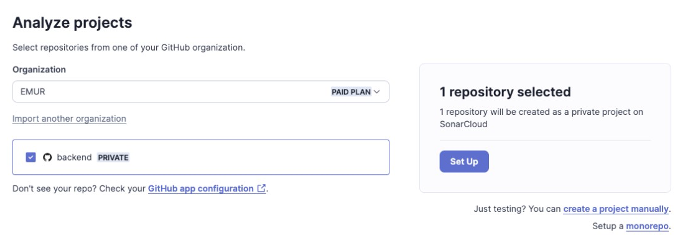
\includegraphics[width=0.7\textwidth]{img/infraestructura/configurar-proyecto.png}
    \caption{Configuración de análisis de proyectos.} \label{Img:Configuración+de+análisis+de+proyectos}
\end{figure} 


Una vez finalizado el análisis primario podemos observar que nos arroja la calidad del código (ver figura~\ref{Img:Resultado+de+análisis+de+código}).

\begin{figure}[h]
    \centering
    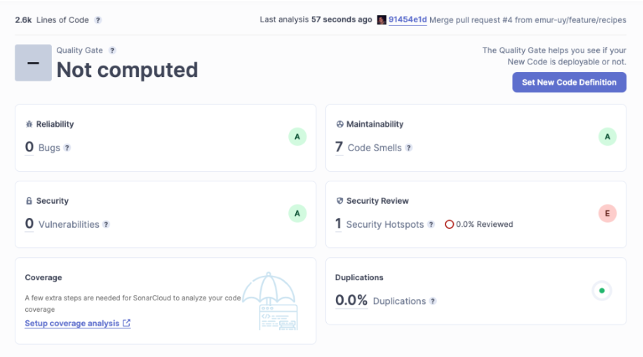
\includegraphics[width=0.7\textwidth]{img/infraestructura/calidad-de-codigo.png}
    \caption{Resultado de análisis de código.} \label{Img:Resultado+de+análisis+de+código}
\end{figure} 

Como podemos ver a continuación nuestro código ha pasado el análisis correctamente y apareciamosque no tiene bugs, ni vulnerabilidades, un bajo porcentaje de code smells y una salud satisfactoria en cuanto a seguridad (ver figura~\ref{Img:Calidad+del+codigo} y ver figura~\ref{Img:Calidad+del+codigo_2}).

\begin{figure}[h]
    \centering
    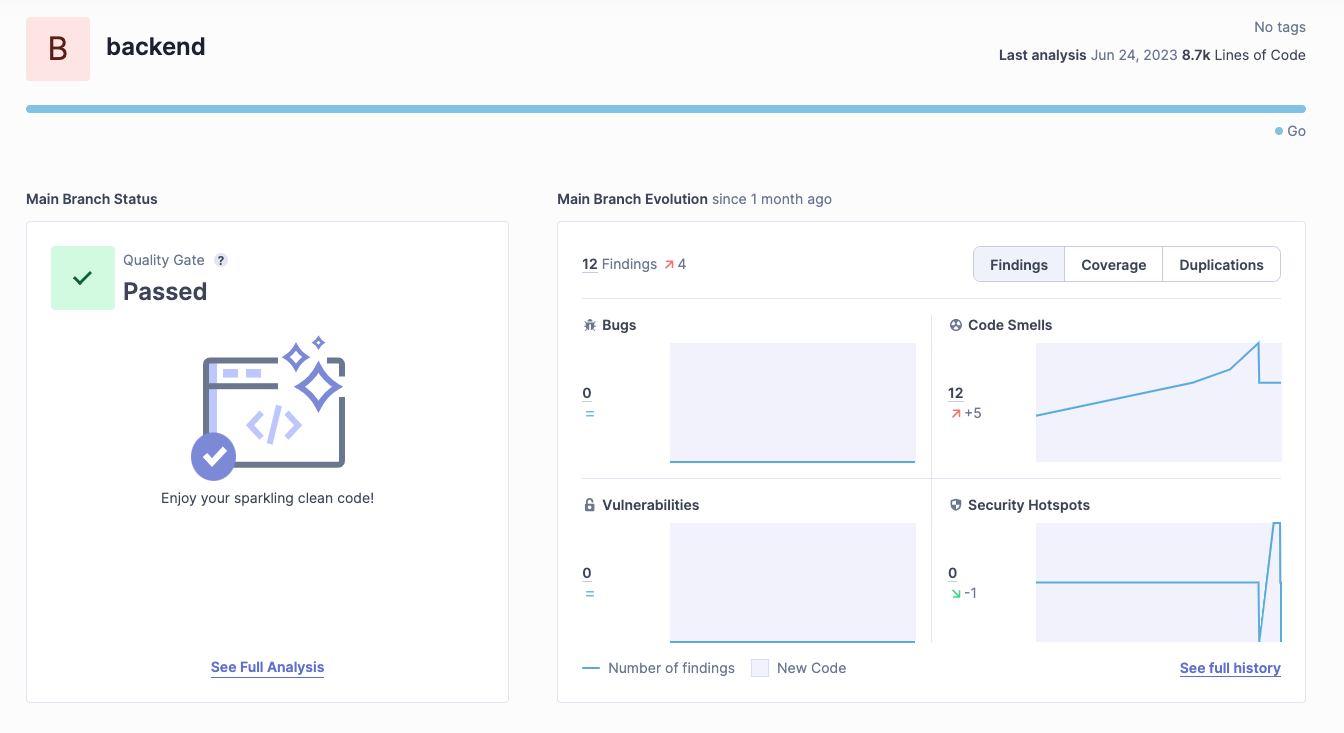
\includegraphics[width=0.8\textwidth]{img/manual/code_sonar_1.png}
    \caption{Resultado de calidad del código parte 1.} \label{Img:Calidad+del+codigo}
\end{figure} 

\begin{figure}[h]
    \centering
    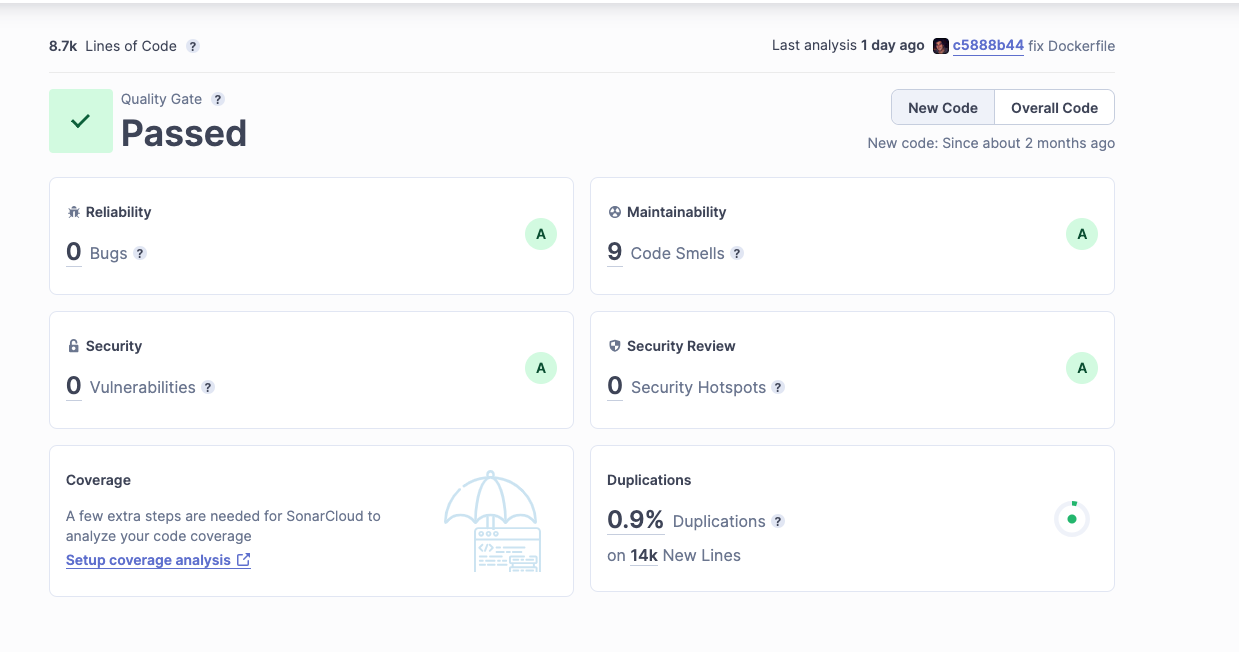
\includegraphics[width=0.8\textwidth]{img/manual/code_sonar.png}
    \caption{Resultado de calidad del código parte 2} \label{Img:Calidad+del+codigo_2}
\end{figure} 

Asimismo se puede ingresar al siguiente enlace para comprobar la calidad del código \href{https://sonarcloud.io/project/overview?id=emur-uy_backend}{SonarCloud}.
\newpage

\section{Github Actions}
Mediante el uso de esta herramienta podemos contar con un servicio de entrega continua, lo que permite subir el código a nuestro repositorio y Github, automáticamente, ejecuta los pipelines desplegando los cambios directamente en el servidor.

En este caso, la receta creada de actions, genera una imagen de Docker y la publica en el repositorio de Docker Hub, seguidamente se conecta al servidor para realizar el despliegue de la nueva imagen de Docker \href{https://hub.docker.com/repository/docker/fabdelgado/api-backend-emur}{Backend} y \href{https://hub.docker.com/repository/docker/fabdelgado/api-chatbot-emur/general}{Chatbot}.

Es de notar que actions de Github necesita ciertas configuración en el repositorio de forma de que pueda conectarse al servidor y al repositorio de Docker Hub, para ello en la sección de settings, en el aparato de seguridad existe una opcion llamada Actions secrets and variables, y es aquí donde procederemos a cargar las variables requeridas (ver tabla~\ref{tab:requisitos-actions}).

\begin{table}[H]
\centering
\begin{tabular}{ll}
\toprule
Variable                     & Valor                           \\
\midrule
\texttt{SERVER\_HOST}       & 134.209.128.98              \\
\texttt{SERVER\_USER}      & root             \\
\texttt{SERVER\_PASSWORD}      & jGqdvXlX2O             \\
\texttt{DEPLOY\_TOKEN}      & Llave pública del servidor             \\
\texttt{DOCKER\_USERNAME}      &  Usuario de Docker Hub      \\
\texttt{DOCKER\_PASSWORD}      & Clave de Docker Hub                \\
\bottomrule
\end{tabular}
\caption{Datos necesarios para Github Actions}
\label{tab:requisitos-actions}
\end{table}

Seguidamente se muestran los pipelines de Github Actions ejecutando las tareas de integración continua sobre el servidor para el backend (ver figura~\ref{Img:Github+Actions+Backend}) y el chatbot (ver figura~\ref{Img:Github+Actions+Chatbot}).

\begin{figure}[h]
    \centering
    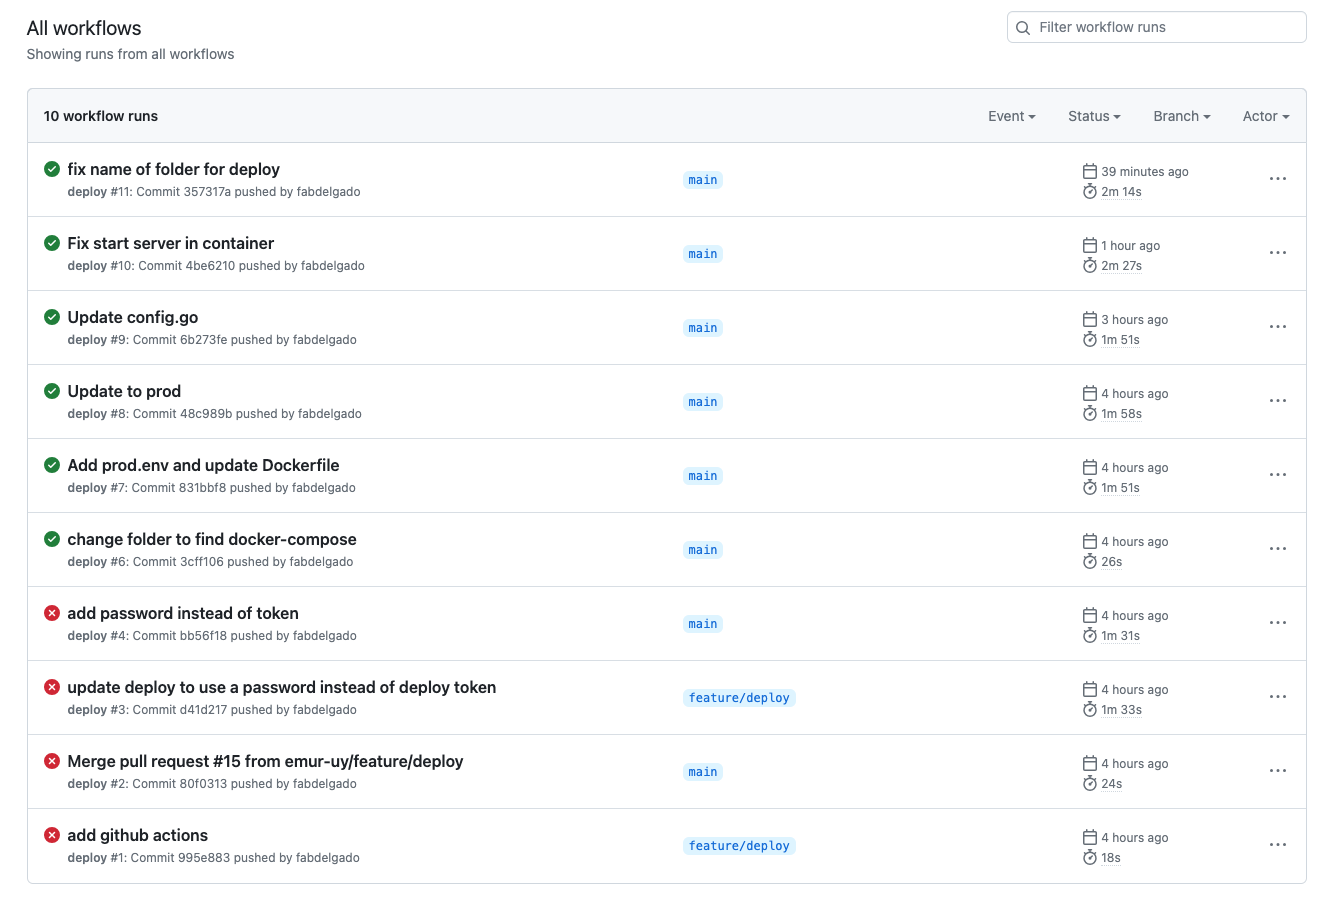
\includegraphics[width=0.7\textwidth]{img/github/ci_backend.png}
    \caption{Ejecución de Github Actions del backend} \label{Img:Github+Actions+Backend}
\end{figure} 

\begin{figure}[h]
    \centering
    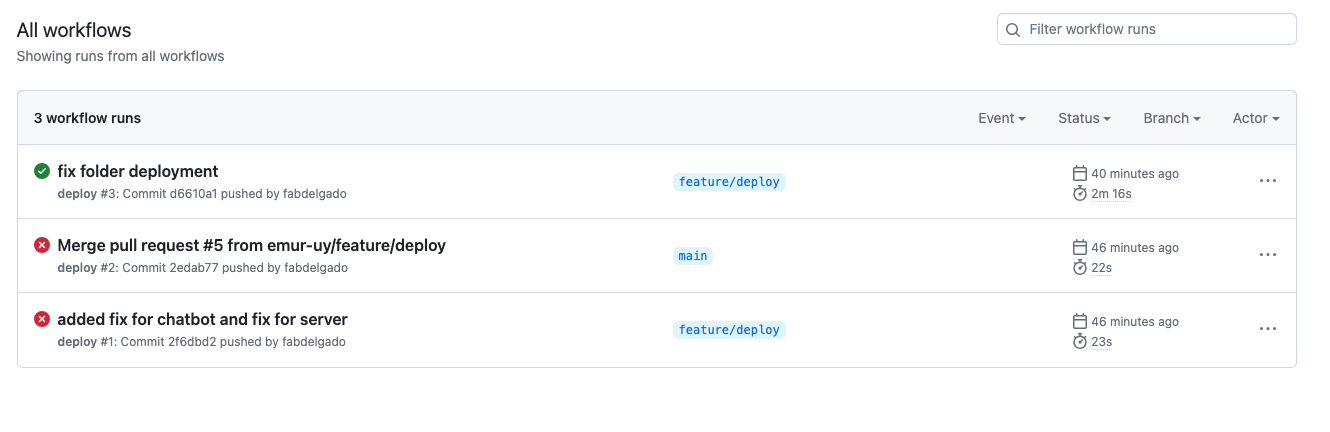
\includegraphics[width=0.7\textwidth]{img/github/ci_chatbot.png}
    \caption{Ejecución de Github Actions del chatbot} \label{Img:Github+Actions+Chatbot}
\end{figure} 

\newpage
\section{Estructura de directorios}

\subsection{Backend}
En el caso de este proyecto de backend la estructura de directorios es muy importante ya que permite organizar el código discriminando en base a las responsabilidades que tiene el sistema desarrollado y a cómo se estructura para mejorar la mantenibilidad en el futuro.

Esta sección detalla cómo está formada la estructura de directorios.

\begin{itemize}
\tightlist
\item
  \texttt{/}: directorio raíz del backend
  \begin{itemize}
  \tightlist
  \item 
    \texttt{makefile}: Archivo utilizado mediante el uso de make para generar las migraciones y ejecutar la creación de las tablas en la base de datos. 
  \item 
    \texttt{run test}: Script que tiene como finalidad la ejecución de los test unitarios.
  \item 
   \texttt{readme}: Contiene la información relevante del proyecto que permite a otros programadores conocer información importante en cuanto al desarrollo.
   \item 
   \texttt{go.mod}: Se encuentran definidas las dependencias del proyecto.
    \item 
   \texttt{go.sum}: Contiene los hashes de cada dependencia para garantizar la integridad.
   \item 
   \texttt{.env}: Archivos donde se alojan las variables de entorno para cada ambiente.
\end{itemize}
\item
  \texttt{/cmd}: contiene los puntos de entrada a la aplicación:
  \begin{itemize}
  \tightlist
  \item 
    \texttt{/api}: Contiene el archivo main, necesario para inicilizar el servidor web. 
  \item  
    \texttt{/worker}: Contiene el archivo main, necesario para inicilizar trabajadores en segundo plano.
    \end{itemize}
    \item
  \texttt{/config}: Contiene un archivo llamado de igual forma que se encarga de cargar las variables que se encuentran en el archivo .env disponibilizándolas a la aplicación.
  \item
  \texttt{/internal}: Contiene los detalles técnicos que necesita la aplicación para funcionar externos a la lógica de negocio de la aplicación.
  \begin{itemize}
  \tightlist
  \item 
    \texttt{/api}: Contiene los controladores y las rutas necesarias para comunicar la aplicación con el afuera.
  \item  
    \texttt{/forecast}: Contiene la implementación para comunicarse con un servicio externo para obtener datos del clima.
  \item  
    \texttt{/repositories}: Contiene los archivos necesarios para realizar la comunicación con repositorios tales como base de datos, storage externo, entre otros.
  \begin{itemize}
  \tightlist
  \item 
    \texttt{/postgresql}: Contiene la implementación abstracta para desacoplar el sistema de la implementación de base de datos.
  \item  
    \texttt{/spaces}: Contiene la implementación para realizar subida, actualización y eliminación de archivos desde un storage externo.
    \end{itemize}
          \item  
    \texttt{/pkg}:
\begin{itemize}
  \tightlist
  \item 
    \texttt{/entity}: Contiene la definición de las entidades también llamadas modelo de dominio.
  \item  
    \texttt{/ports}: Esta carpeta contiene las interfaces necesitarias para interconectar el servicio con la base de datos.
  \item  
    \texttt{/services}: Contiene la lógica de negocio.
    \end{itemize}
    \end{itemize}
    \texttt{/migrations}: Contiene los archivos SQL para generar las tablas o actualizarlas.
    \end{itemize}

\subsection{Chatbot}
En el caso de la estructura de directorios para el chatbot, se trata de una estructura muy simple ya que está basada en ejecución de scripts. A continuación se detallan los archivos más importantes.

\begin{itemize}
\tightlist
\item
  \texttt{/}: directorio raíz del chatbot
  \begin{itemize}
  \tightlist
  \item 
    \texttt{alembic}: Contiene las migraciones para la base de datos.
  \item 
    \texttt{db\_docs}: Contiene la estructura generada por FAISS de vectores.
  \item 
   \texttt{api.py:}: Script que disponibiliza la API.
   \item 
   \texttt{engine.py:} Script motor que genera los vectores para FAISS a partir de la información extraída de la base de datos.
    \item 
    \texttt{chatbot.py:}Script que se encarga de buscar el vector mas cercano a la pregunta del usuario y interactuar con ChatGPT para generar la respuesta.
    \item 
    \texttt{scrapper.py:} Script encargado de navegar por el sitio web extrayendo y formateando la información en crudo para que luego se procesada por el engine.
   \item 
   \texttt{.env}: Archivos donde se alojan las variables de entorno para el ambiente.
    \item 
   \texttt{requirements.txt}: Se encuentran definidas las dependencias del proyecto .
    \item 
   \texttt{startup.sh}: Inicia el servidor gunicorn usando hilos.
    \end{itemize}
\end{itemize}

 
\section{Compilación, instalación y ejecución del proyecto}
Esta sección tiene como objetivo brindar los conocimientos básicos que permitan entender cómo trabajar con el proyecto, realizar modificaciones o evolucionarlo en el tiempo.

 \subsection{Entorno de desarrollo}
Es necesario contar con las siguientes herramientas aqui descriptas:
 
 \begin{itemize}
  \tightlist
  \item Visual Studio Code
  \item Golang
  \item Python
  \item Git
  \item Table Plus
  \item Postman
  \item Make
\end{itemize}

\subsubsection{Visual Studio Code}\label{visual-studio-code}

Visual Studio Code es un editor de código de fuente abierto, gratuito, y multiplataforma con una gran cantidad de extensiones disponibles, y que se utiliza para desarrollar aplicaciones en una variedad de lenguajes de programación como Python, JavaScript, TypeScript, Golang, entre otros. En este sentido, no se requirió de licencia para el editor de código facilitando su uso.

Para abrir el proyecto en Visual Studio Code primero debemos proceder a realizar la descarga de este software (ver figura~\ref{Img:Descarga+de+Visual+studio+code}).
Para ello nos dirigimos a la \href{https://code.visualstudio.com/}{web oficial}. 

\begin{figure}[h]
    \centering
    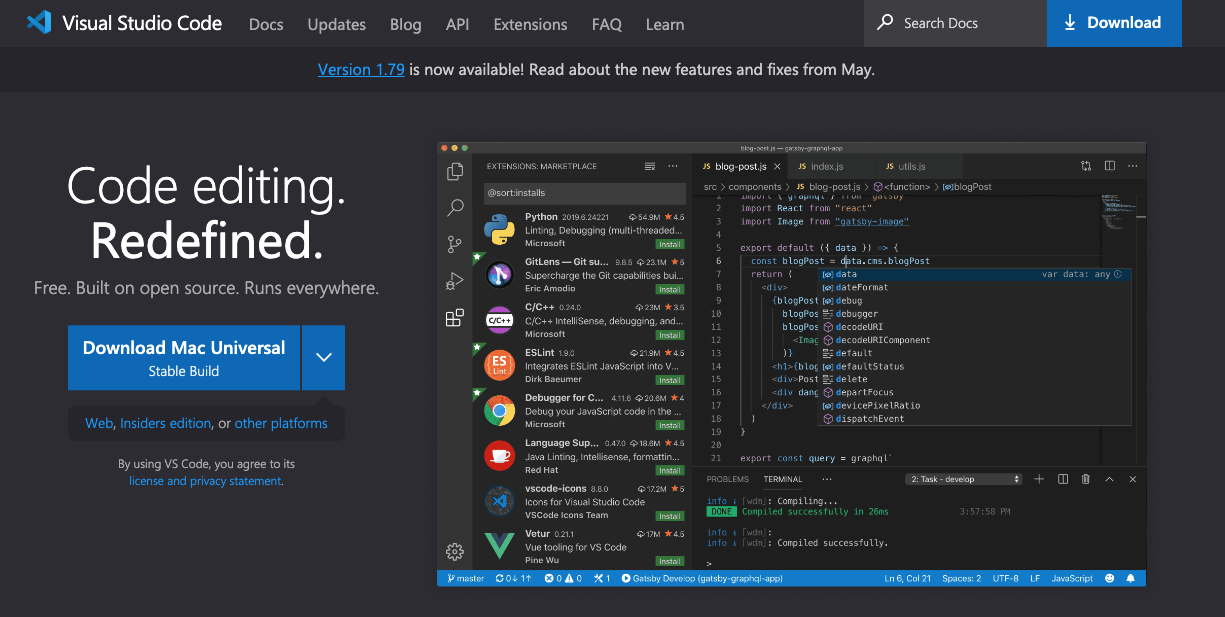
\includegraphics[width=0.7\textwidth]{img/manual/visual-studio-code.png}
    \caption{Descarga de Visual Studio Code} \label{Img:Descarga+de+Visual+studio+code}
\end{figure} 

Para instalarlo, basta con arrastrar el software hacia la carpeta aplicaciones (ver figura~\ref{Img:Instalar+Visual+studio+code}).
\begin{figure}[h]
    \centering
    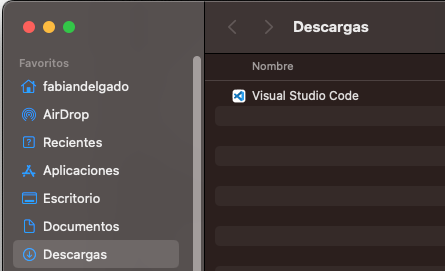
\includegraphics[width=0.7\textwidth]{img/manual/instalar-visual-studio-code.png}
    \caption{Instalar Visual studio code} \label{Img:Instalar+Visual+studio+code}
\end{figure} 

Una vez que lo tenemos instalado en nuestro sistema y abrimos el sofware, hacemos clic en Archivo -> abrir carpeta y ya tendremos nuestro código en el editor.

\subsubsection{Golang}\label{golang}
Golang, también conocido como Go, es un lenguaje de programación de código abierto que se utiliza principalmente para aplicaciones de sistemas, redes y servicios web. Cuenta con compilación estática, lo que significa que el código se compila antes de que se ejecute, y utiliza una recolección de basura eficiente, por lo que los recursos del sistema se emplean de una mejor forma. Asimismo, Golang tiene un modelo de concurrencia incorporado que permite crear aplicaciones que pueden manejar múltiples tareas al mismo tiempo sin afectar el rendimiento. 

Para realizar la instalación, se debe ingresar a la sección de descargas del sitio web oficial de \href{https://go.dev/dl/}{Golang} y seleccionar la versión más reciente (ver figura~\ref{Img:Lista+de+versiones+de+Golang}).

\begin{figure}[h]
    \centering
    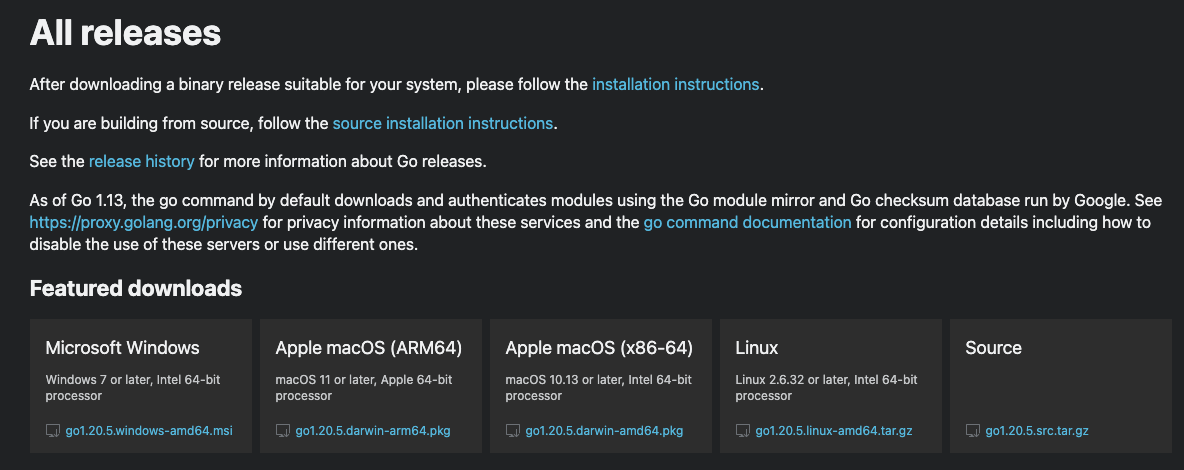
\includegraphics[width=0.7\textwidth]{img/manual/releases.png}
    \caption{Lista de versiones de Golang} \label{Img:Lista+de+versiones+de+Golang}
\end{figure} 

Una vez descargado el paquete de software que instalará Golang en el sistema, basta con iniciarlo y presionar siguiente hasta que se complete la instalación (ver figura~\ref{Img:Instalación+de+Golang}).

\begin{figure}[h]
    \centering
    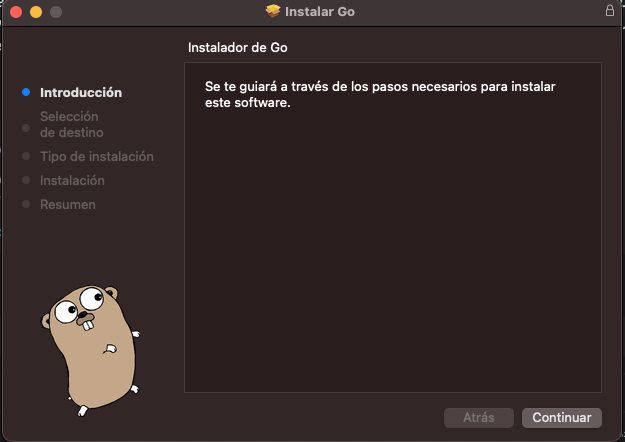
\includegraphics[width=0.7\textwidth]{img/manual/instalacion.png}
    \caption{Instalación de Golang} \label{Img:Instalación+de+Golang}
\end{figure} 

\subsubsection{Python}\label{python}
Python es un lenguaje de programación de alto nivel, orientado a objetos, que presenta una gran cantidad de características similares con otros lenguajes como C++, Java, Modula-3 y Scheme, por lo que ofrece un equilibrio óptimo entre lo práctico y lo conceptual. Es fácil de usar por su sintaxis simple, clara y concisa que facilita su aprendizaje y el mantenimiento de proyectos de gran envergadura, al mismo tiempo, que ofrece un entorno multiplataforma que puede ser ejecutado en diversos sistemas operativos.

Para la instalación de \href{https://www.python.org/downloads/}{Python} hay que ir a su web de descargas, donde la misma detectará nuestra versión de sistema operativo permitiéndonos descargar la última disponible (ver figura~\ref{Img:Lista+de+versiones+de+Python}).

\begin{figure}[h]
    \centering
    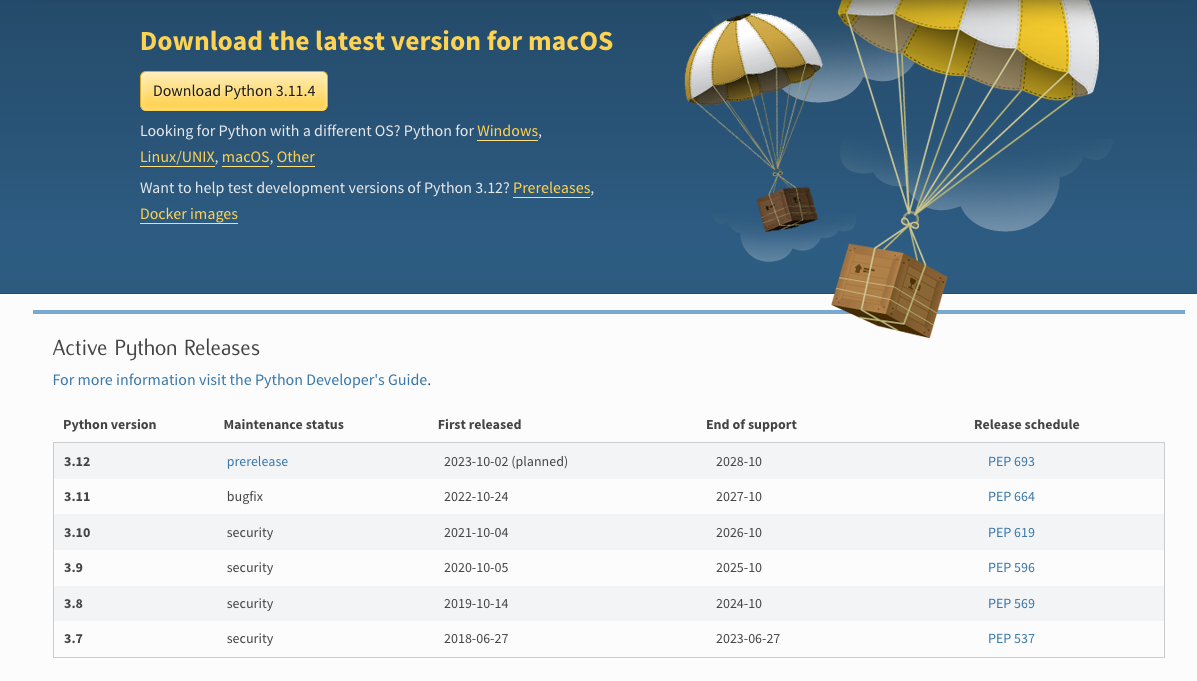
\includegraphics[width=0.5\textwidth]{img/manual/lista-versiones-python.png}
    \caption{Lista de versiones de Python} \label{Img:Lista+de+versiones+de+Python}
\end{figure} 
Una vez que ya contamos con el paquete para instalarlo en nuestro sistema, procedemos a ejecutarlo y damos continuar hasta finalizar la instalación (ver figura~\ref{Img:Instalación+de+Python}).

\begin{figure}[h]
    \centering
    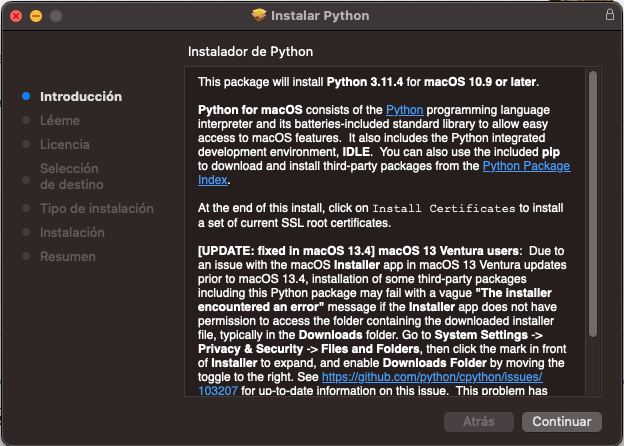
\includegraphics[width=0.7\textwidth]{img/manual/instalacion-python.png}
    \caption{Instalación de Python} \label{Img:Instalación+de+Python}
\end{figure} 

\newpage


\subsubsection{Git}\label{git}
Git es un programa destinado al control de versiones software en el que se registran los cambios producidos en el mismo, facilitando la integración de código por parte de cualquiera de los integrantes del proyecto. En Git cada desarrollador tiene una copia completa del repositorio, pudiendo trabajar de forma independiente sin depender de un servidor central. Por otro lado, Git utiliza un modelo de ramificación y fusión que permite a los desarrolladores trabajar en paralelo en diferentes características o correcciones de errores sin interferir entre sí.

Para poder clonar el repositorio del proyecto y trabajar con él, es necesario contar con Git instalado en el sistema. 
Para instalarlo, podemos navegar a la web de SourceForge y proceder a descargar el instalable de \href{https://sourceforge.net/projects/git-osx-installer/files/git-2.23.0-intel-universal-mavericks.dmg/download?use_mirror=autoselect}{Git} (ver figura~\ref{Img:Instalación+de+Git}).

\begin{figure}[h]
    \centering
    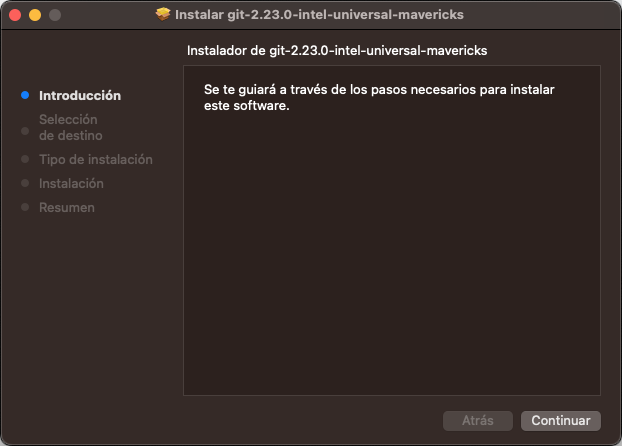
\includegraphics[width=0.7\textwidth]{img/manual/instalar-git.png}
    \caption{Instalación de Git} \label{Img:Instalación+de+Git}
\end{figure} 

\newpage

Luego de este proceso ya podemos clonar el \href{https://github.com/emur-uy}{repositorio} utilizando la url del mismo. Para este fin ejecutamos el siguiente comando git clone -b main git@github.com:emur-uy/backend.git (ver figura~\ref{Img:Clonación+de+repositorio+desde Github}).

\begin{figure}[h]
    \centering
    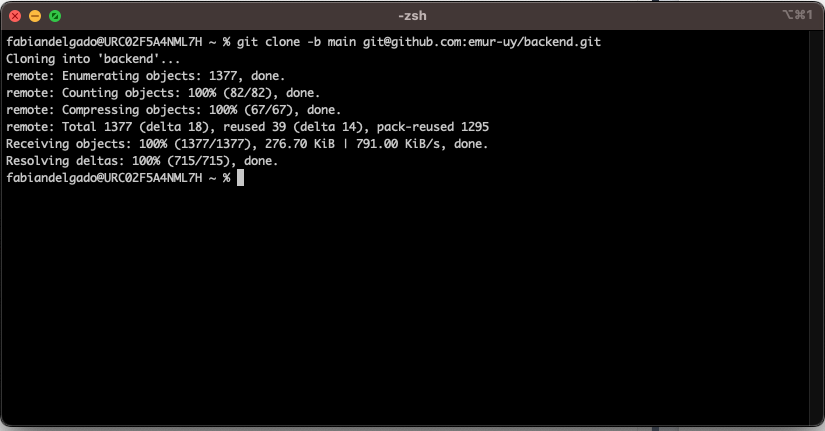
\includegraphics[width=0.7\textwidth]{img/manual/git-clonado.png}
    \caption{Clonación de repositorio desde Github} \label{Img:Clonación+de+repositorio+desde Github}
\end{figure} 


\subsubsection{Table Plus}\label{table-plus}
TablePlus es un software de gestión de bases de datos con una interfaz gráfica de usuario intuitiva y fácil de usar. Permite a los usuarios conectarse y administrar múltiples bases de datos de manera eficiente y en una sola aplicación, así como navegar por bases de datos relacionales de forma cómoda y sencilla. Ofrece una serie de características útiles como autocompletado de código SQL, la búsqueda de texto completo y la vista de esquema, que hacen que la gestión de bases de datos sea más eficiente y productiva. 

Para instalarlo debemos navegar hasta su \href{https://tableplus.com/}{sitio web}, una vez alli procedemos a hacer click en el botón de descargar (ver figura~\ref{Img:Descarga+de+software+Table+Plus}).

\begin{figure}[h]
    \centering
    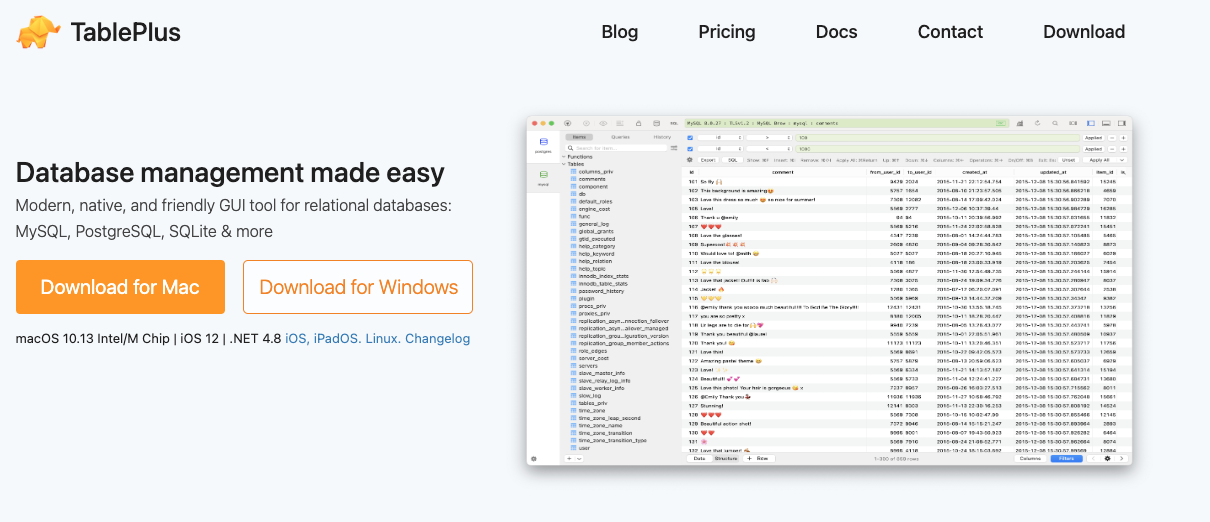
\includegraphics[width=0.7\textwidth]{img/manual/table-plus.png}
    \caption{Descarga de software Table Plus.} \label{Img:Descarga+de+software+Table+Plus}
\end{figure} 

Para instalarlo basta con abrir el instalador y arrastra el ícono hacia la carpeta de aplicaciones (ver figura~\ref{Img:Instalación+Table+Plus}).

\begin{figure}[h]
    \centering
    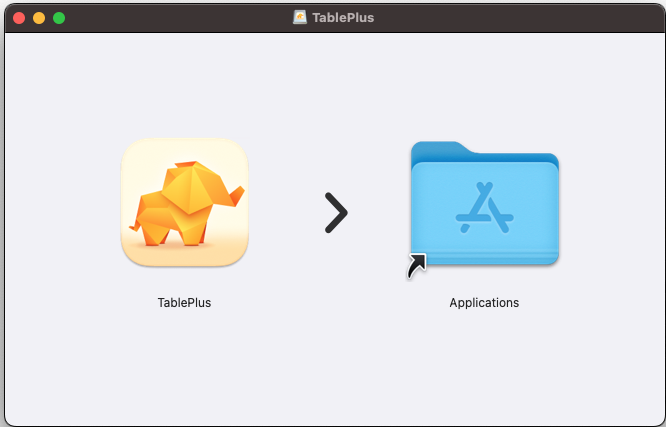
\includegraphics[width=0.7\textwidth]{img/manual/instalacion-table-plus.png}
    \caption{Instalación Table Plus.} \label{Img:Instalación+Table+Plus}
\end{figure} 

Luego ya podemos configurar nuestra instancia de base de datos remota. Para ello, una vez iniciado el software Table Plus completamos con lo datos que se solicitan conforme se aprecia en la siguiente imagen (ver tabla~\ref{tab:requisitos-table-plus}).

\begin{table}[H]
\centering
\begin{tabular}{ll}
\toprule
Campo                     & Valor                           \\
\midrule
\texttt{Name}       & Emur DEV              \\
\texttt{Host}      & db-postgresql-nyc1-56709-do-user-9370728-0.b.db.ondigitalocean.com             \\
\texttt{User}      & emur             \\
\texttt{Password}      &  ver archivo .env      \\
\texttt{Database}      & dev\_emur\_backend           \\
\texttt{Port}      & 25060             \\
\bottomrule
\end{tabular}
\caption{Datos de acceso a la base de datos de desarrollo}
\label{tab:requisitos-table-plus}
\end{table}

A continuación, podemos observar cómo queda configurado en la ventana de Table Plus, listo para conectarse y validando en color verde que fue posible establecer conexión con los datos provistos (ver figura~\ref{Img:Configuración+de+base de+datos+en+Table+Plus}).

\begin{figure}[h]
    \centering
    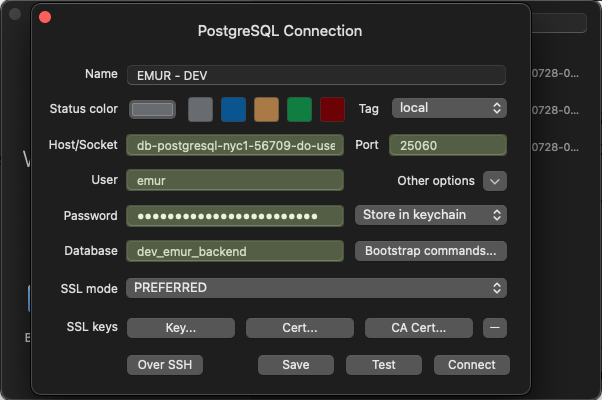
\includegraphics[width=0.7\textwidth]{img/manual/connect-table-plus.png}
    \caption{Configuración de base de datos en Table Plus.} \label{Img:Configuración+de+base de+datos+en+Table+Plus}
\end{figure} 


\section{Documentación de las APIs}\label{postman}

\subsection{Postman}\label{postman}
Postman es una herramienta de prueba de APIs que permite a los desarrolladores crear, probar, documentar y compartir colecciones de APIs de manera rápida y fácil. En ella, los programadores pueden crear solicitudes HTTP personalizadas y enviarlas a cualquier API en línea o local, y de varias formas, incluyendo GET, POST, PUT, DELETE y PATCH, lo que permite ahorrar tiempo y recursos.

Postman nos permite realizar las pruebas sobre los endpoints de las APIs a medida que queremos corroborar datos o probar nuevos desarrollos sobre las mismas.
Para poder obtener Postman debemos navegar a la zona de \href{https://www.postman.com/downloads/}{descarga} de su sitio web (ver figura~\ref{Img:Descarga+de+Postman})

\begin{figure}[h]
    \centering
    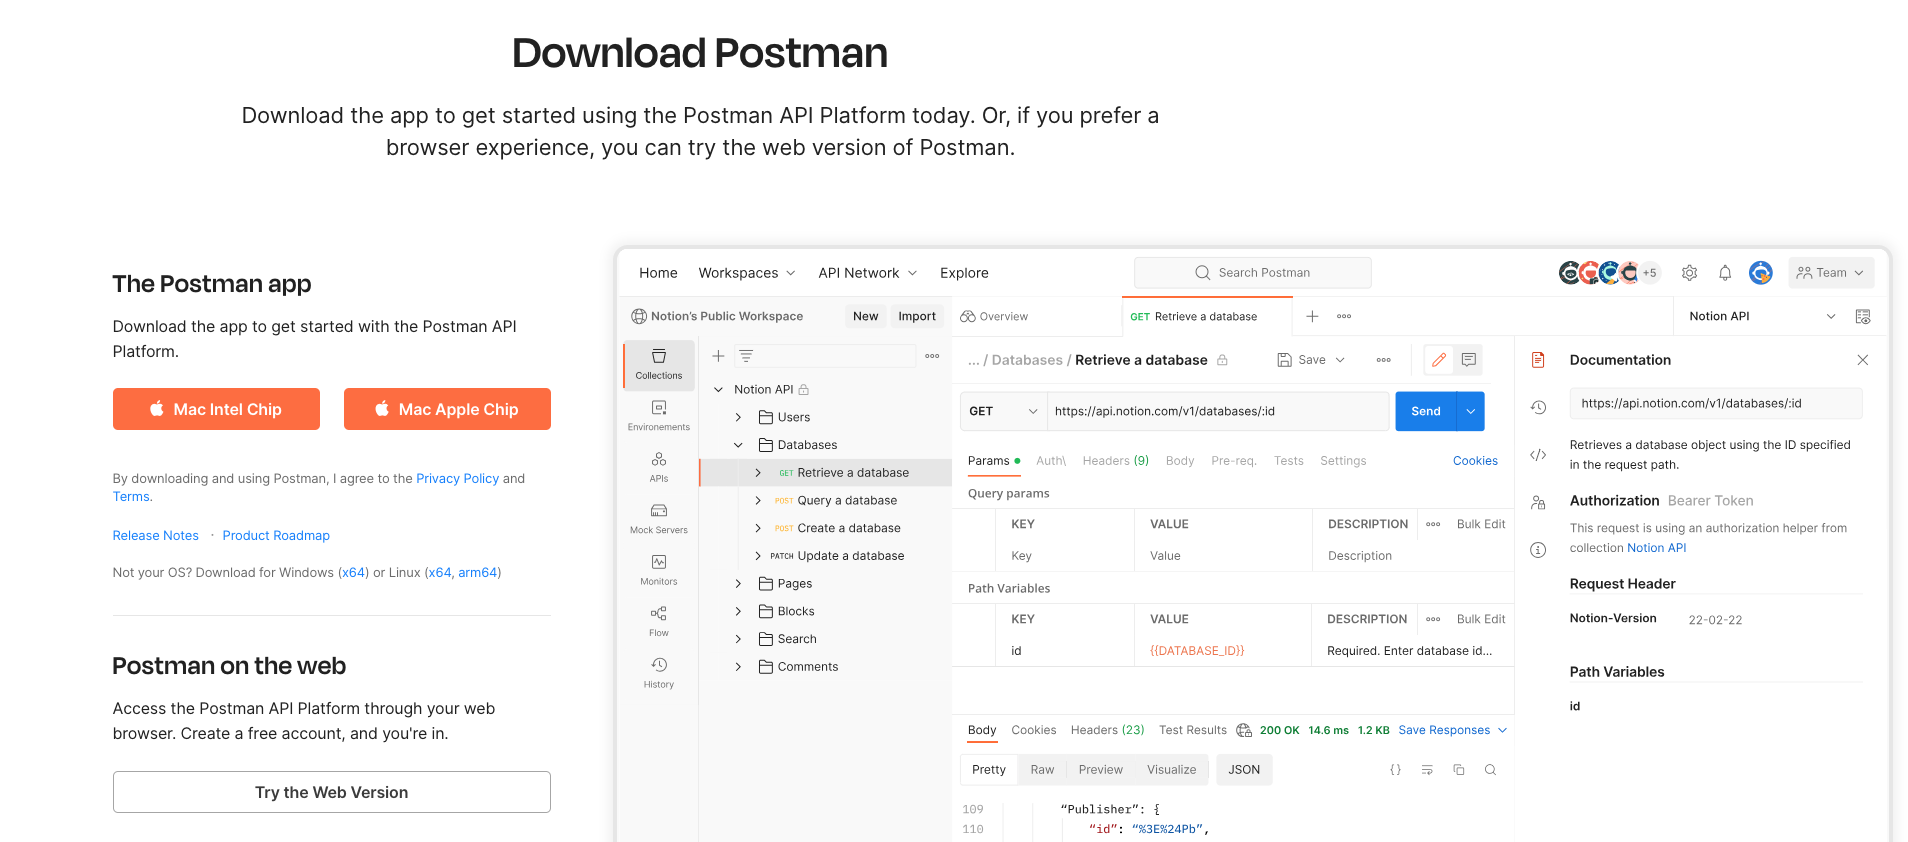
\includegraphics[width=0.9\textwidth]{img/manual/postman-descargas.png}
    \caption{Descarga de Postman.} \label{Img:Descarga+de+Postman}
\end{figure} 

Una vez alli procedemos a descargar la versión que corresponde a nuestro sistema operativo, luego de la descarga procedemos a instalarlo arrastrando el ícono a la carpeta de aplicaciones
(ver figura~\ref{Img:Instalación+de+Postman})

\begin{figure}[h]
    \centering
    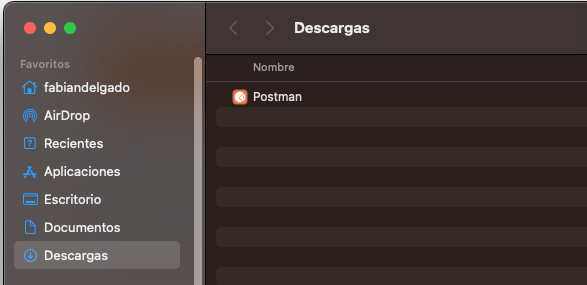
\includegraphics[width=0.7\textwidth]{img/manual/postman-instalar.png}
    \caption{Instalación de Postman} \label{Img:Instalación+de+Postman}
\end{figure} 

Seguidamente, se necesita importar la colección que contiene los endpoints de las APIs desarrolladas del backend. Abrimos Postman y nos dirigimos a File -> Import, arrastramos el zip que contiene dichas colecciones y que se encuentra subido al repositorio bajo la carpeta Postman (ver figura~\ref{Img:Abrir+colección+de+Postman})


\begin{figure}[h]
    \centering
    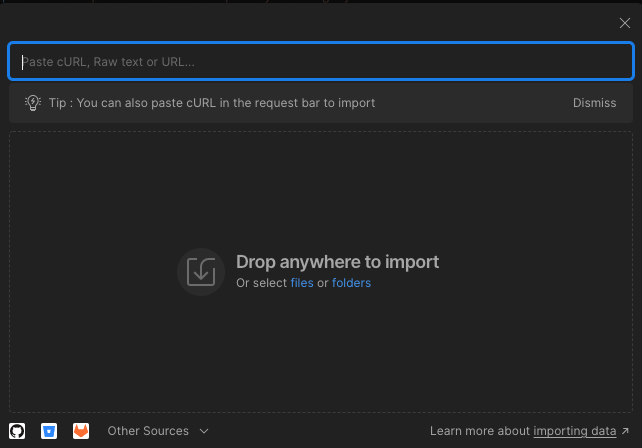
\includegraphics[width=0.7\textwidth]{img/manual/abrir-coleccion-postman.png}
    \caption{Abrir colección de Postman} \label{Img:Abrir+colección+de+Postman}
\end{figure} 

\subsection{Swagger}\label{swagger}
Swagger hace referencia a un conjunto de herramientas, especificaciones y reglas destinadas a la documentación de las APIs. Es fácil de utilizar dada su simplicidad, y la documentación generada puede implementarse directamente en la automatización de procesos dependientes de APIs. Swagger permite hacer pruebas de APIs, y sus elementos, y ofrece compatibilidad con Java, Javascript, Ruby, PHP y Actionscript.

Además del uso de Postman, tal como vimos anteriormente para documentar las APIs, támbien se ha implementado en el proyecto el uso de Swagger permitiendo así contar con una documentación siempre disponible para hacer más fácil el desarrollo de la futura aplicación móvil.

Se puede ingresar a la documentación de Swagger mediante los siguientes links:

\begin{itemize}
\tightlist
\item
  \texttt{Backend}: \href{http://134.209.128.98:8080/docs/index.html}{http://134.209.128.98:8080/docs/index.html}
 \item 
  \texttt{Chatbot}: \href{http://134.209.128.98:5005/apidocs/}{http://134.209.128.98:5005/apidocs/}
\end{itemize}

\begin{figure}[h]
    \centering
    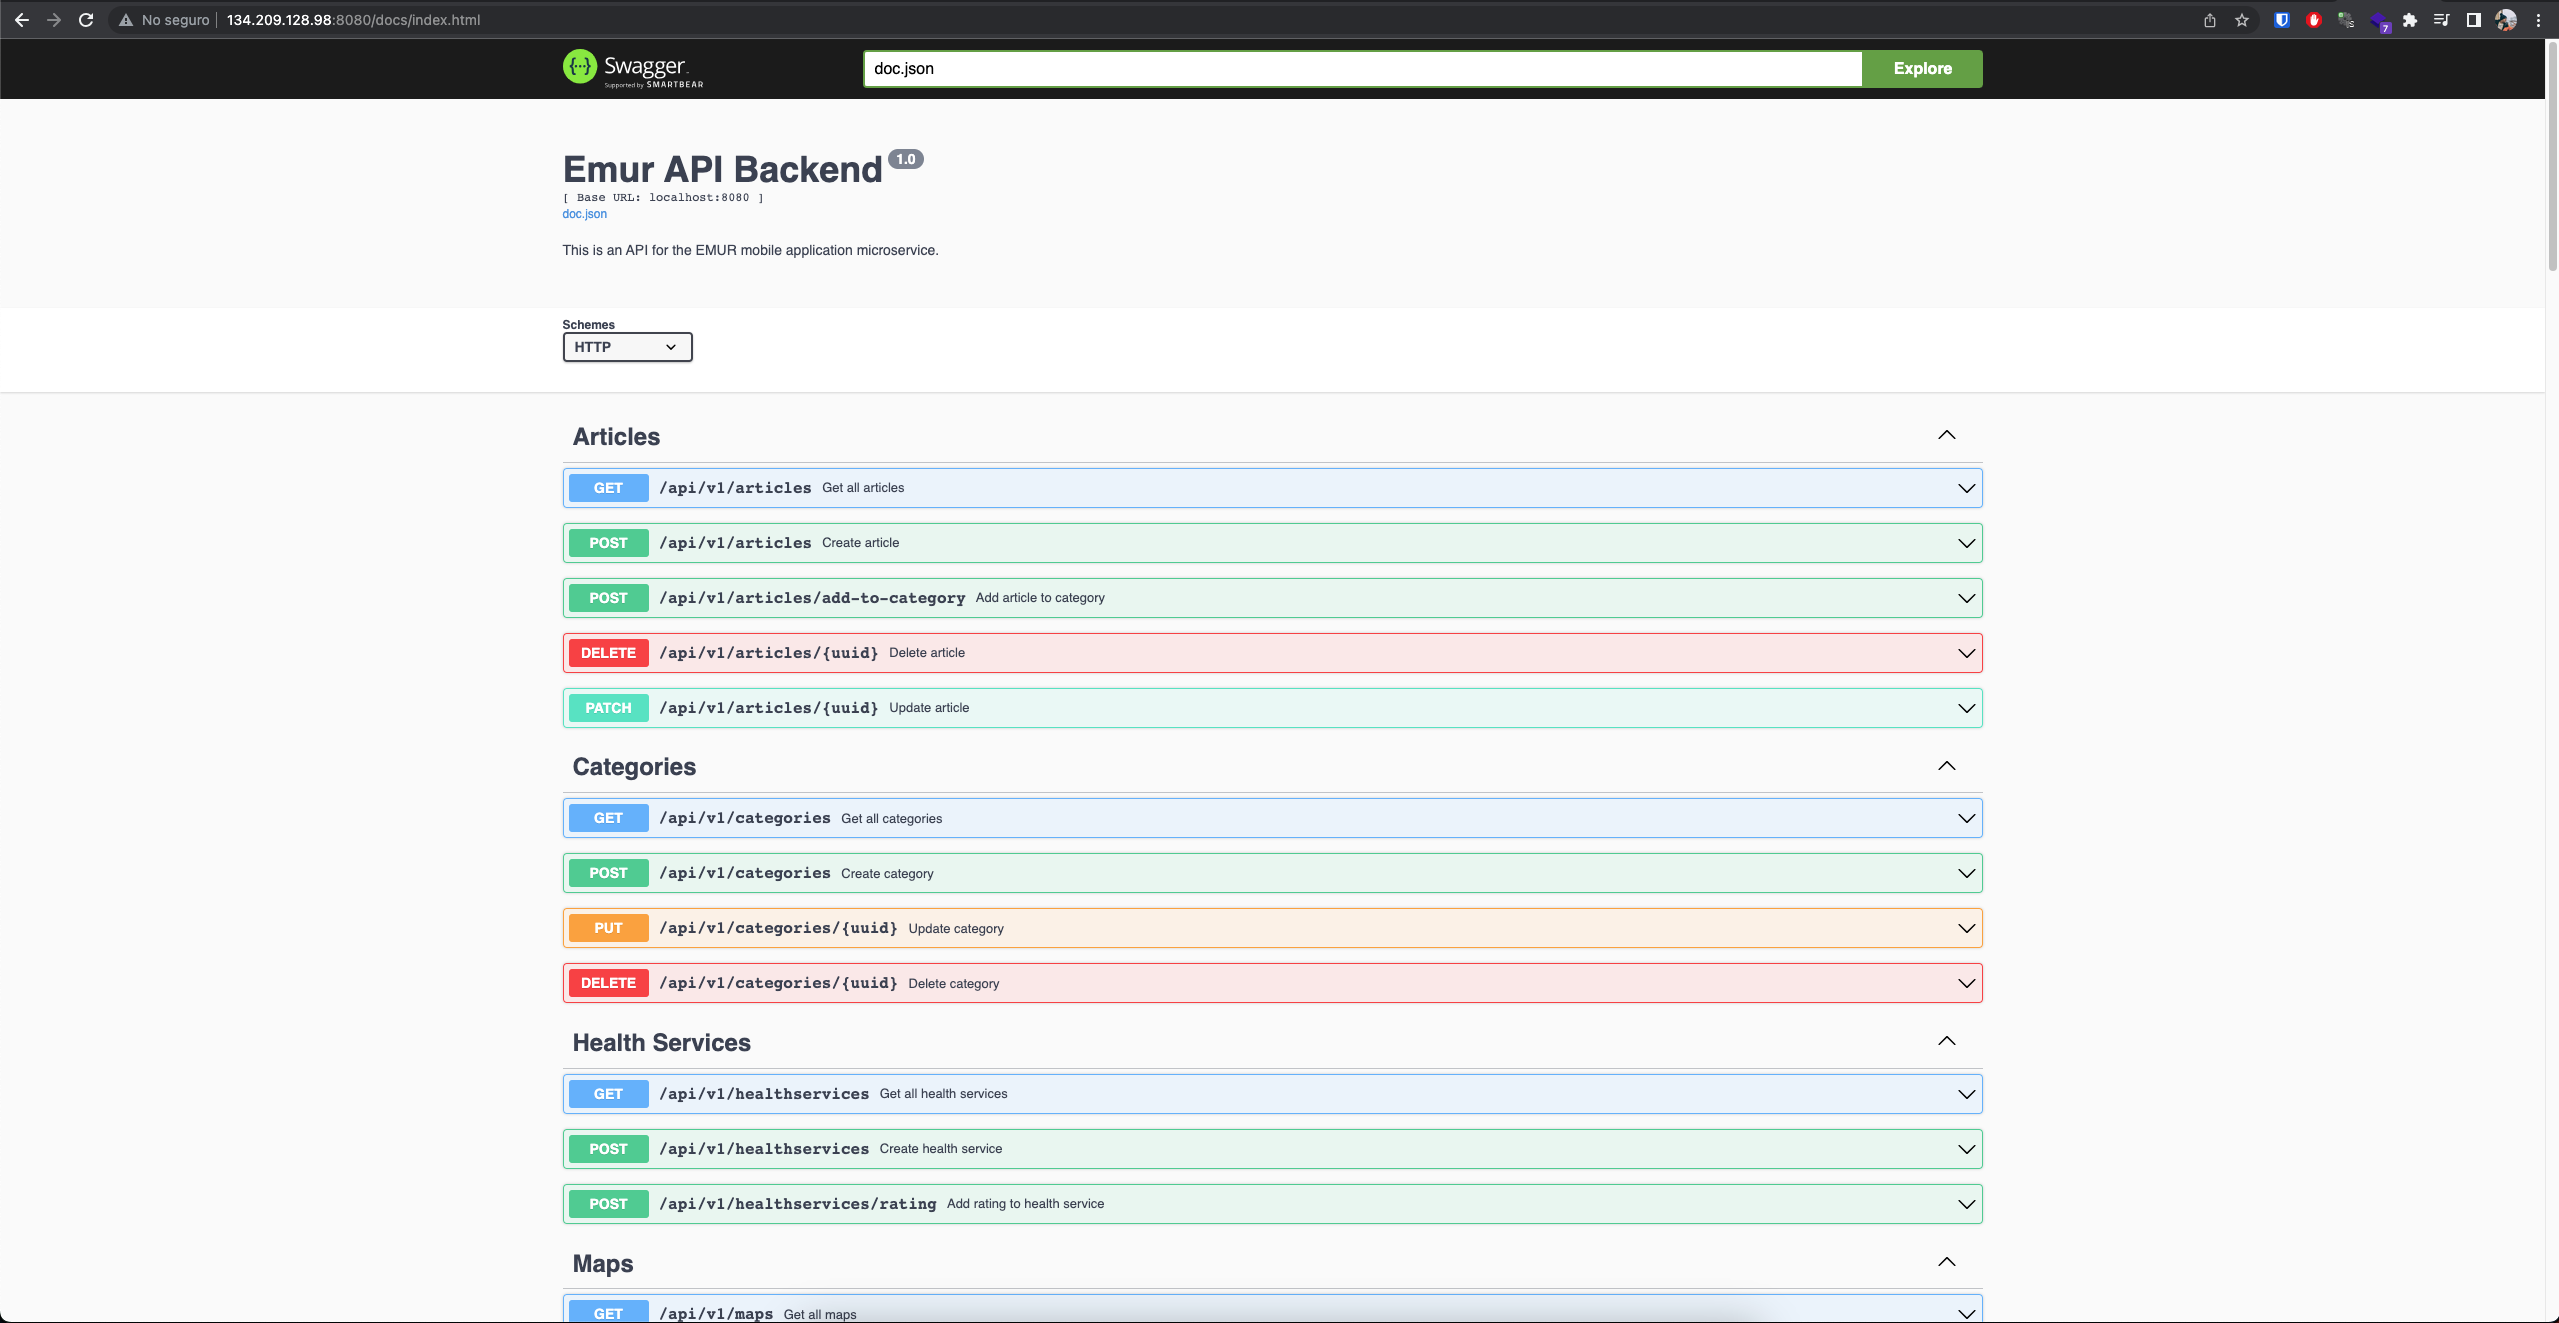
\includegraphics[width=0.7\textwidth]{img/infraestructura/swagger_backend.png}
    \caption{Swagger de Backend} \label{Img:Swagger+backend}
\end{figure} 

\begin{figure}[h]
    \centering
    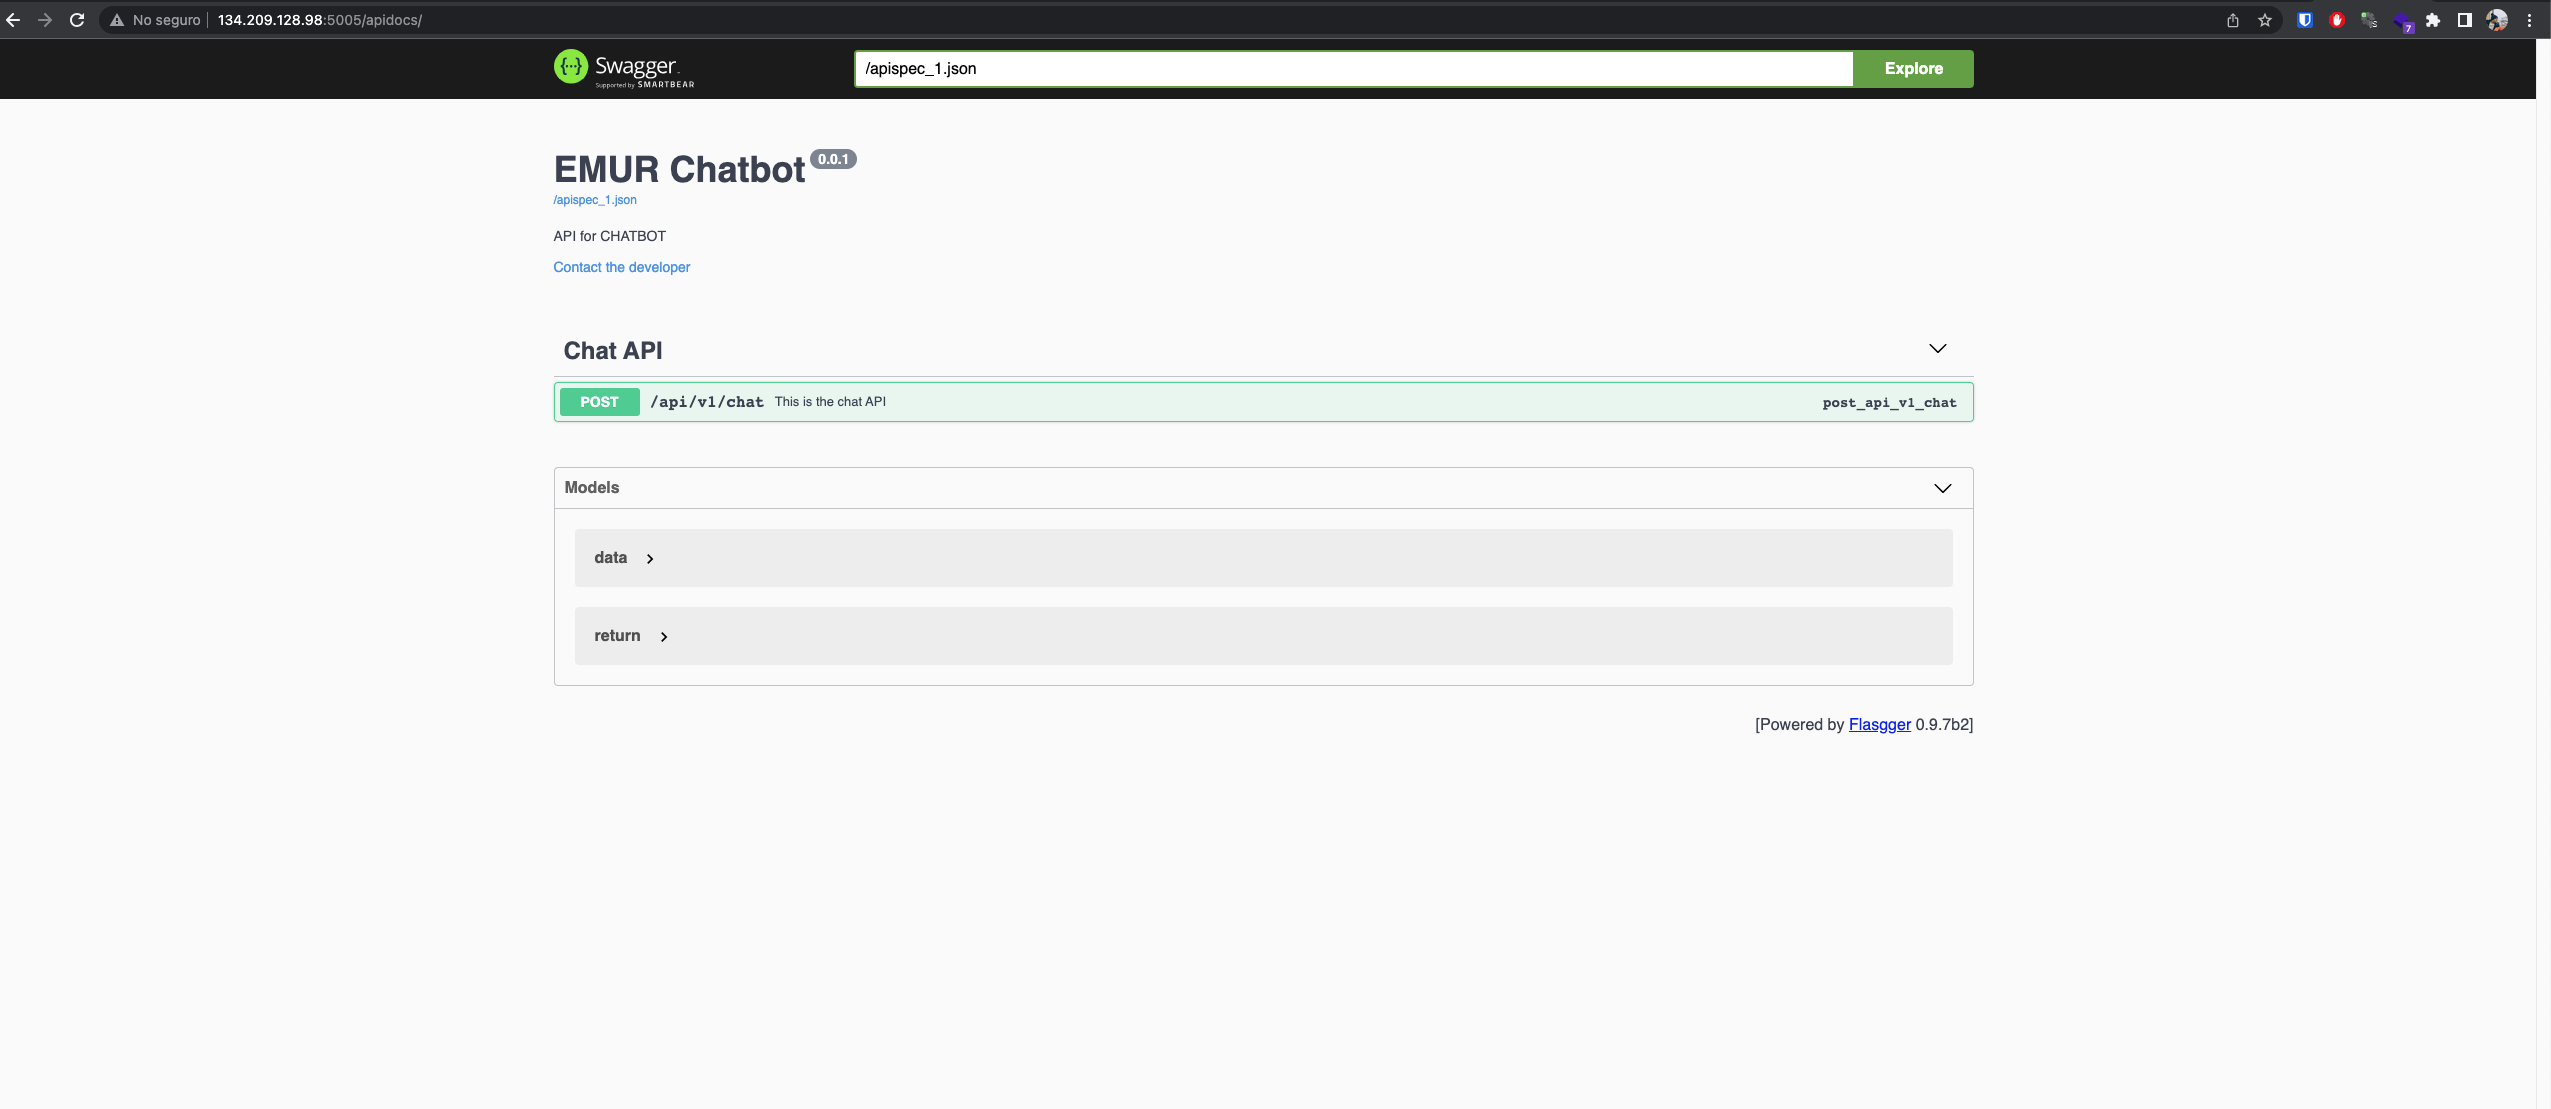
\includegraphics[width=0.7\textwidth]{img/infraestructura/swagger_chatbot.png}
    \caption{Swagger de Chatbot} \label{Img:Swagger+chatbot}
\end{figure} 

\newpage
\section{Pruebas del sistema}
Para comprobar el correcto funcionamiento del backend, se realizaron tanto pruebas unitarias como funcionales ya que esto permite asegurar la mantenibilidad, correcto funcionamiento ante futuros cambios y corroborar que el sistema continua operando e interoperando con la futura aplicación móvil.

\subsection{Test unitarios}
La finalidad de los test unitarios es asegurar de manera atómica que los módulos desarrollados en el software continúan funcionando ante cambios realizados. Ello permite asegurar que el código actual siga funcionando con la adición del nuevo.

Para realizar las pruebas se utilizó el paquete de Golang llamado testify en conjunto con el framework de Golang GIN, esto permite realizar test y probar el comportamiento de la APIs.
Amerita mencionar que, para las pruebas, se utilizó mocking, ya que permite simular el acceso de información como si de una base de datos se tratara, haciendo posible probar su comportamiento a diferentes situaciones.

En este backend se realizaron 18 test unitarios sobre los servicios asegurando, de esta forma, la lógica de negocio del sistema.

\subsection{Ejecución de los test unitarios}
Para la ejecución de los test unitarios, Golang nos propone el comando "go test -v service/*\_test.go. Dado que éste sólo habilitaba su uso de forma unitaria por cada archivo creado, se procedió a implementar un script que permitiese ejecutar todo el set de pruebas.
Para utilizar dicho script se necesita contar con permisos de ejecución, lo que puede efectuarse a través del comando chmod x ./run\_test.sh.

En las siguientes capturas podemos ver todos los test ejecutándose satisfactoriamente
(ver figura~\ref{Img:Resultado+de+test+parte+1} y ver figura~\ref{Img:Resultado+de+test+parte+2}).

\begin{figure}[h]
    \centering
    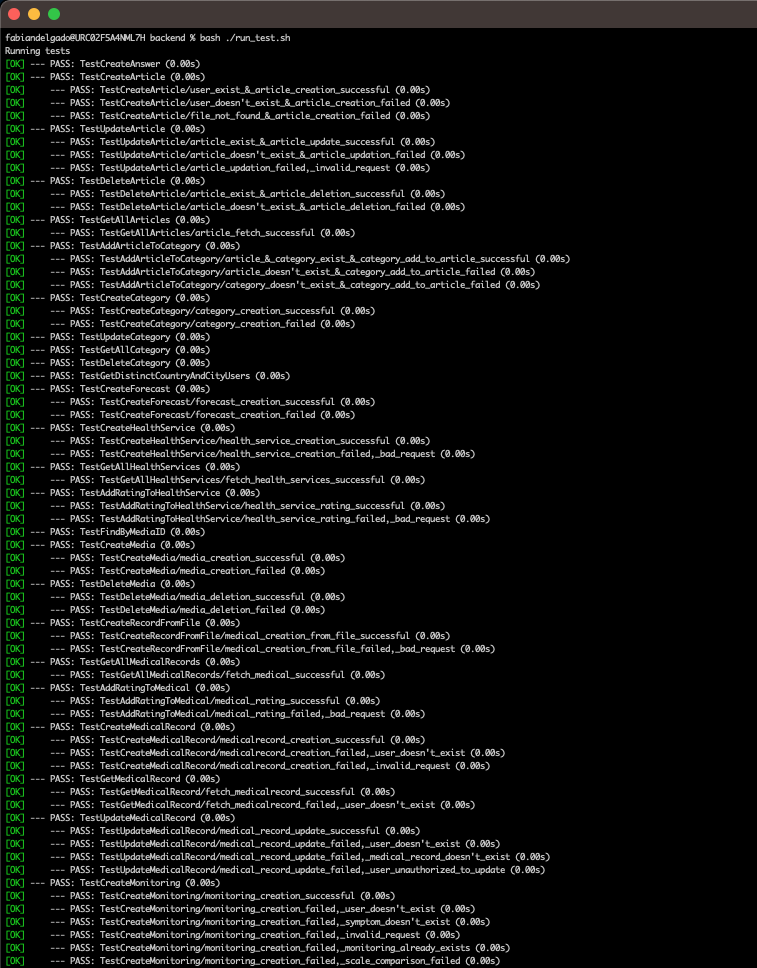
\includegraphics[width=0.5\textwidth]{img/manual/test_parte_1.png}
    \caption{Resultado de test parte 1.} \label{Img:Resultado+de+test+parte+1}
\end{figure} 


\begin{figure}[h]
    \centering
    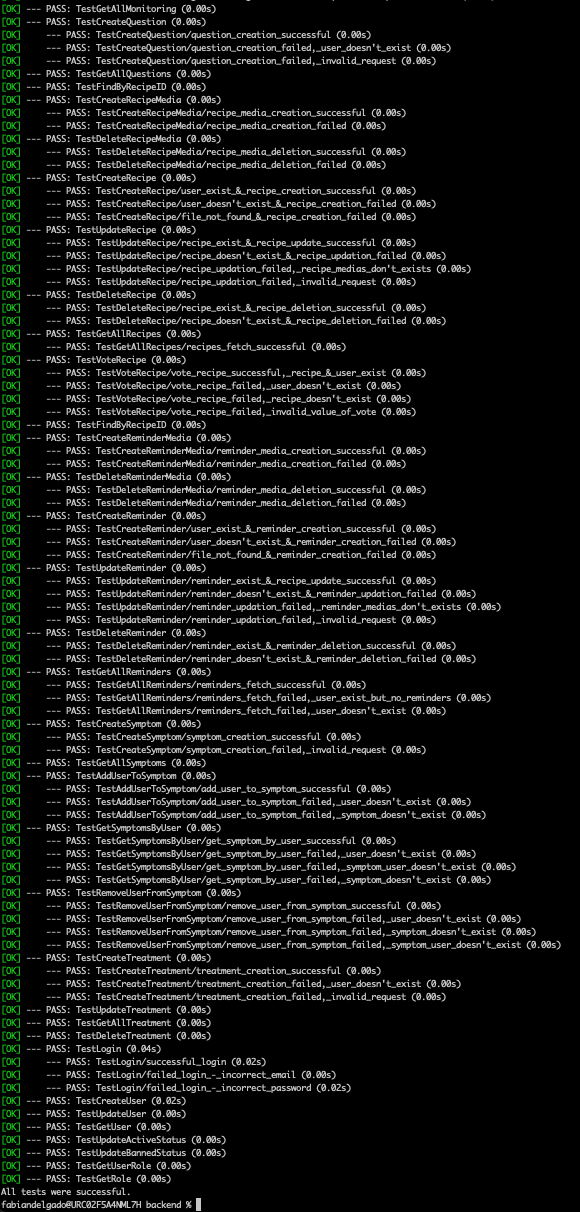
\includegraphics[width=0.5\textwidth]{img/manual/test_parte_2.png}
    \caption{Resultado de test parte 2.} \label{Img:Resultado+de+test+parte+2}
\end{figure} 

\subsection{Test funcionales}

Los test funcionales se encargan de asegurar que los datos de salida del sistema se encuentren operando de acuerdo a lo esperado en la especificaciones.
Asimismo, se centran en realizar las pruebas de interacciones tal como lo haría un usuario del sistema y nos permiten, además, asegurar que el sistema, de cara al usuario, se encuentra funcionando adecuadamente.

En el caso de este proyecto, al tratarse de APIs que serán el backend de la futura aplicación móvil, las pruebas funcionales se realizaron a través de Postman.

La manera de automatizarlas, para evitar probar endpoint por endpoint, ha sido utilizar la funcionalidad Runner de Postman que permite realizar programáticamente la evaluación y asertividad de los datos que espera nuestro frontend.

\begin{figure}[h]
    \centering
    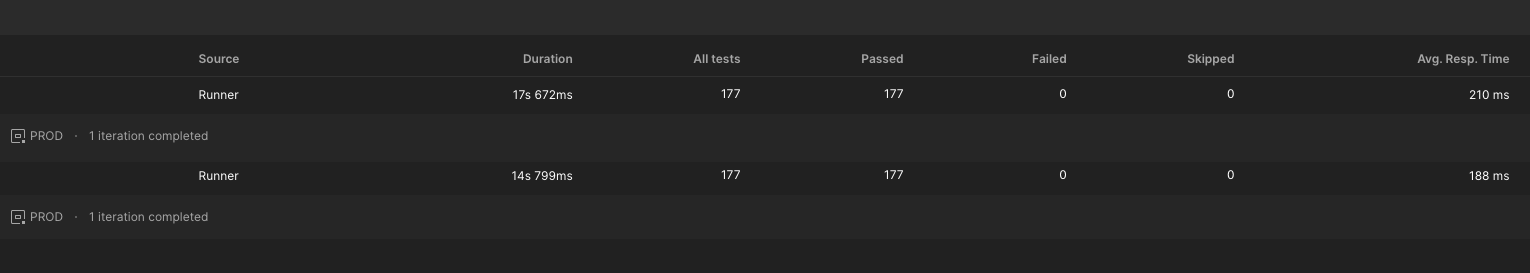
\includegraphics[width=1.0\textwidth]{img/manual/test_admin.png}
    \caption{Resultado de la ejecucíon de los test automatizados de admin.} \label{Img:Resultado+de+test+admin}
\end{figure} 

\begin{figure}[h]
    \centering
    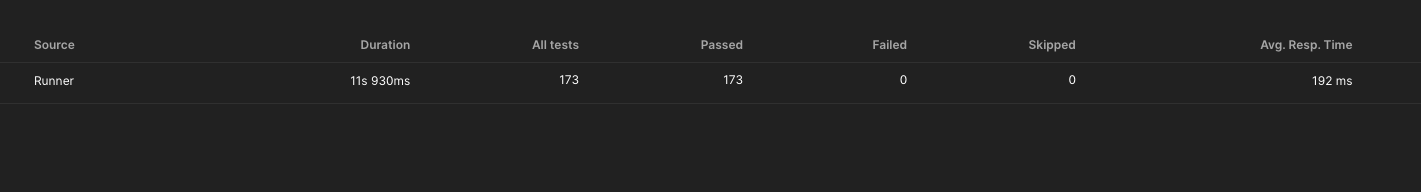
\includegraphics[width=1.1\textwidth]{img/manual/test_usuario.png}
    \caption{Resultado de la ejecucíon de los test automatizados de usuario.} \label{Img:Resultado+de+test+usuario}
\end{figure} 
\newpage
\subsection{Pruebas de estrés}
Estas pruebas se encargan de realizar test de rendimiento sobre el sistema para así determinar su robustez en condiciones de alta concurrencia. Para ello, el sistema se sobrecarga con solicitudes para emular una cantidad de usuarios concurrentes.
De esta forma, se busca identificar los límites del sistema para encontrar cualquier problema que pudiera surgir en cuanto a la performance, ya sea de servidor, código o de acceso a la base de datos para disminuir los tiempos y evitar cuellos de botella.
\begin{figure}[h]
    \centering
    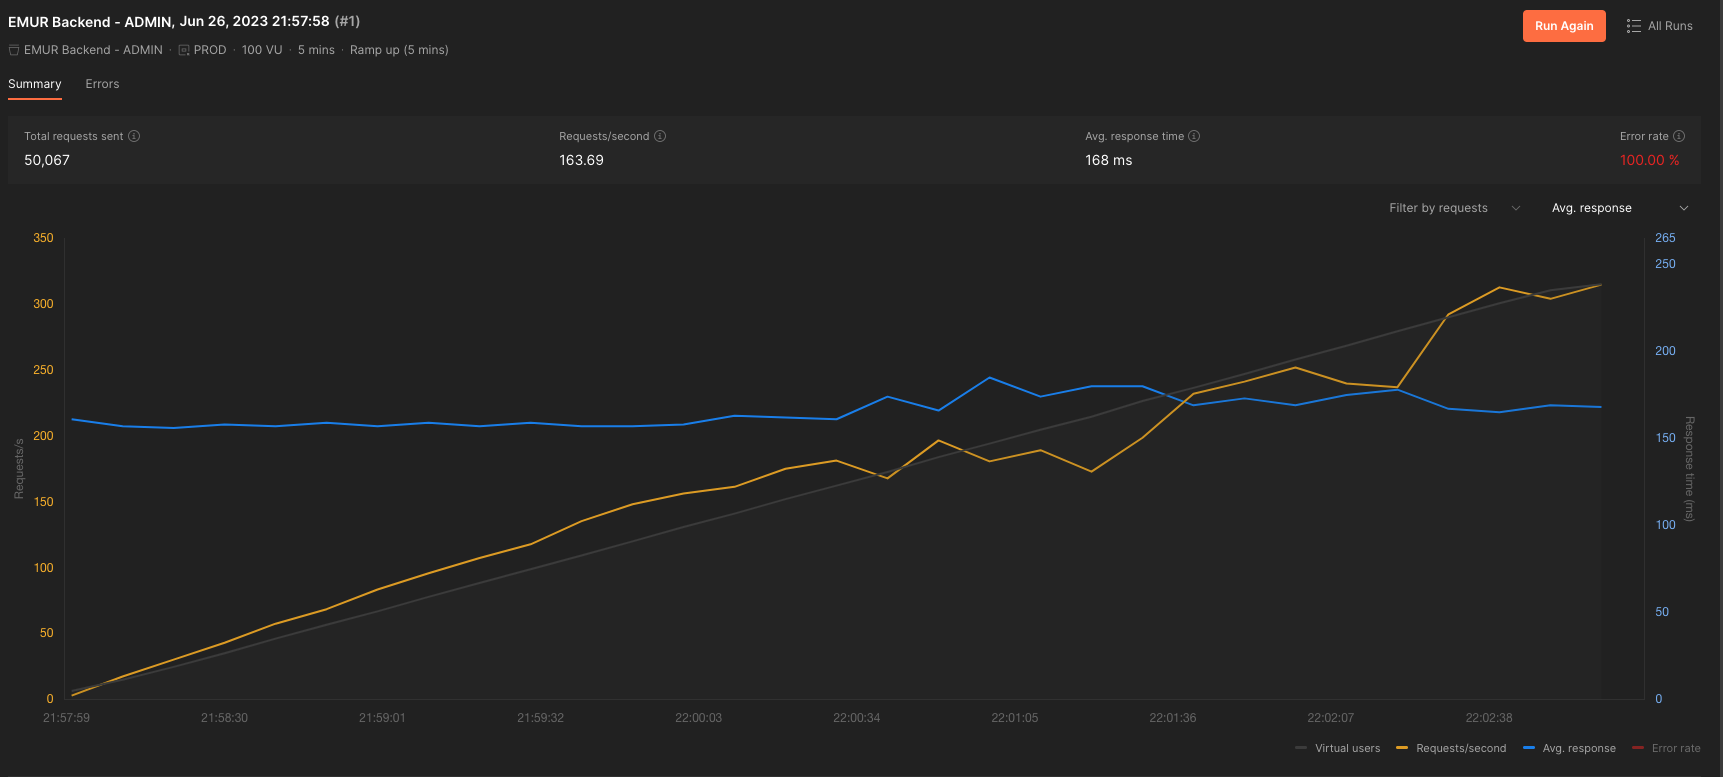
\includegraphics[width=1.0\textwidth]{img/manual/test_de_stress.png}
    \caption{Resultado de la ejecución de los test de stress.} \label{Img:Resultado+de+test+stress}
\end{figure} 



